% !TEX root = ../main.tex
%
%\begin{savequote}[8cm]
%	\textlatin{Le doute n'est pas une état bien agréable, mais l'assurance est un état ridicule.}
%	
%	Doubt is not a very agreeable status, but certainty is a ridiculous one.
%	\qauthor{--- Voltaire}
%\end{savequote}


\chapter{Probabilistic Machine Learning}
\label{chp:bayes}

In this chapter we will provide a high-level introduction to  some of the core approaches to
machine learning.  We will distinguish between discriminative and generative approaches,
outlining some of the key features that indicate when problems are more suited to one approach
or the other.  Our focus then settles on probabilistic generative approaches, which
will be the main focus of this thesis.  We will explain how the \emph{Bayesian paradigm} provides
a powerful framework for generative machine learning that allows us to combine data with existing
expertise.  We will then go on to show how \emph{graphical models} can be used as a convenient
framework to express Bayesian models and extract important features.  
We continue by introducing the main counterpart to the Bayesian approach -- frequentist
approaches -- and present arguments for why neither alone provides the full story
In particular, we will outline the fundamental underlying
assumptions made by each approach and explain why the differing suitability of these
assumptions to different tasks means that both are  essential tools in the machine learning
arsenal, with many problems requiring both Bayesian and frequentist elements in their analysis.
Though much of the focus of this thesis will be on Bayesian approaches, understanding their limitations
is essential for understanding when the methods we discuss should be used and critically when they
should not.  We finish the chapter by discussing some of the key practical challenges for Bayesian modeling.

% !TEX root = ../main.tex

\section{Discriminative vs Generative Machine Learning}
\label{sec:bayes:discrim}

In some machine learning applications, huge quantities of data are available that dwarf the information
that can be provided from human expertise.  In such situations, the main challenge is in processing
and extracting all the desired information from the data to form a useful characterization,
typically an artifact providing accurate predictions at previous unseen inputs. 
Such problems are typically suited to \emph{discriminative} 
machine learning approaches~\citep{breiman2001statistical,vapnik1998statistical}, such as neural
networks~\citep{rumelhart1986learning,bishop1995neural}, 
support vector machines~\citep{cortes1995support,scholkopf2002learning}, and decision tree 
ensembles~\citep{breiman2001random,rainforth2015canonical}.  Discriminative machine learning approaches
focus on directly learning a predictive model: given training data $\mathcal{D} = \left\{x_n,y_n\right\}_{n=1}^N$
they learn a parametrized mapping $f_{\theta}$ from the inputs $x \in \mathcal{X}$ to the 
outputs $y\in\mathcal{Y}$ that can 
be used directly to make predictions 
for new inputs $\tilde{x} \notin \left\{x_n\right\}_{n=1}^N$.  \emph{Training}
uses the data $\mathcal{D}$ to estimate optimal values of the parameters $\theta^*$. \emph{Prediction}
at a new input $\tilde{x}$ involves applying the mapping with the optimal parameters giving an estimate for the output
$\tilde{y} = f_{\theta^*}(\tilde{x})$.  Perhaps the simplest example of this is linear regression: one finds
the hyperplane that best represents the data and then uses this hyperplane to interpolate or extrapolate
to previously unseen points.  
As a more advanced example, in a neural network one uses training to learn the
weights of the network, after which prediction can be done by running the network forwards.  

There are many intuitive reasons to take a discriminative machine learning 
approach.  Perhaps most compelling is the
idea that if our objective is prediction, then it is simplest to solve that problem directly, rather
than try and solve some more general problem such as learning an underlying generative 
process~\citep{vapnik1998statistical,breiman2001statistical}. Furthermore, if sufficient
data is provided, discriminant approaches can be spectacularly successful in term of predictive
performance.  Discriminant methods are typically highly flexible and can capture intricate structure in the data that
would be hard or even impossible to establish manually.  Many approaches can also be run with little
or no input on behalf of the user, delivering state-of-the-art performance when used
``out-of-the-box'' with default parameters~\citep{rainforth2015canonical}.  

However, this black-box nature is also often their downfall.  Discriminative methods typically make
such weak assumptions about the underlying process that is difficult to impart prior knowledge
or domain-specific expertise.  This can be disastrous if insufficient data is available, as the data
alone is unlikely to possess the required information to make adequate predictions.  Even when
substantial data is available, there may be significant prior information available that needs to be
exploited for effective performance.  For example, in time series modelling the sequential nature
of the data is critically important information~\citep{liu1998sequential}, while in vision tasks the 
knowledge that scenes are generated from objects can be invaluable~\citep{kulkarni2015picture}.
Many problems also increase in complexity as more data is added -- ``big data'' problems are often
actually a collection, or sometimes hierarchy, of many small problems, such that the complexity of the
required parametrization increases are more data is added.  Consider, for example, modeling interactions in
a social network.  Adding a new user into the model increases the amount of data, but also
requires the model to grow and accommodate the new user~\citep{ravasz2003hierarchical}.  In
this situation it is essential to
use an approach that respects the structure of the model, while the amount of data available
for each individual user is often quite small, such that it will essential to use prior information
by transferring insights gathered from some users to others.  Therefore even for such large-scale
problems, the inflexibility of many discriminative approaches to incorporate known characteristics
of the target problem can be problematic.

Not only does the black-box nature of many discriminative methods restrict the level of
human input that can be imparted on the system, it often restricts the amount of insight
and information that can be extracted from the system once trained.  The parameters in most discriminative
algorithms do not have physical meaning that can be queried by a user, making their operation
difficult to interpret and hampering the process of improving the system through manual
revision of the algorithm.  Furthermore, this typically makes them inappropriate for more
statistics orientated tasks, where it is the parameters themselves which are of interest, rather
than the ability for the system itself to make predictions.  For example, the parameters may
have real-world physical interpretations we wish to learn about.

Most discriminative methods are also poor at providing realistic uncertainty estimates.
Because they are typically trained in a manner that optimizes the parameters to minimize
some loss criterion (e.g. the predictive error), they do not, in general, encode any uncertainty
in either their parameters or the subsequent predictions.  Though many methods can
produce uncertainty estimates either as a by-product or from a post-processing step,
these are typically heuristic based, rather than stemming naturally from a statistically
principled estimate of the target uncertainty distribution.   This lack of reliable uncertainty
estimates can lead to overconfidence and can make discriminative methods inappropriate in
many scenarios.  It can also reduce the composability of discriminative methods within
larger systems, as information is lost when only providing a point estimate.
Not representing uncertainty in the parameters can also restrict the power of the resultant
models, compared with approaches that can average over different possible parameter values.

These shortfalls mean that many tasks instead call for a \emph{generative} machine learning
approach~\citep{ng2002discriminative,bishop2006pattern}.  Rather than directly learning a 
predictor, generative methods look to explain the observed data using a \emph{probabilistic model}.
Whereas discriminative approaches aim only to make predictions, generative approaches model
how the data is actually generated; they model the joint probability $p(X,Y)$ of the inputs 
$X$ and outputs $Y$.  By comparison, we can think of discriminative approaches as
only modeling the outputs given the inputs $p(Y|X)$.  

A key upshot of this difference
is that generative approaches generally make stronger modeling assumptions about the problem.  Though
this can be problematic when the model assumptions are wrong and is often unnecessary in
the limit of large data, it is essential for combining prior information with data
and therefore for constructing systems that exploit application-specific human expertise.
In the words of the great George Box, ``\textit{all models are wrong, but some are useful}''
\citep{box1979robustness,box2005statistics}.  In a way, this is a self-fulfilling statement: a model for
any real phenomena
is by definition an approximation and so is never exactly correct no matter how powerful.  However,
it is still an essential point that is all too often forgotten, particularly by academics trying to convince
the world that only their approach is correct.  Only in artificial situations can we construct exact models
and so we must remember, particularly in generative machine learning, that the first, and often largest,
error is in our original mathematical abstraction of the problem.  On the other hand, real situations
have access to finite and often highly restricted data, so it is equally preposterous to suggest that a
method is superior simply due to better asymptotic behavior in the limit of large data, or that if our approach
does not work then the solution is simply to get more data.\footnote{It should, of course, be noted
	that the availability of data is typically the biggest bottleneck in machine learning.  At times, it feels 
	like the machine learning community would we well served to remember that the differences in performance between
	machine learning approaches is often, if not usually, dominated by variations in the inherently difficultly of the
	problem, which is itself not usually known up front, rather than differences between approaches.}  As such, the ease of which domain-specific
expertise can be included in generative approaches is often essential to achieving effective performance
on real world tasks.

To highlight the difference between discriminative and generative machine learning, we consider the
example of the differences between logistic regression (a discriminative classifier) and na\"{i}ve Bayes 
(a generative classifier).  We will consider the binary classification case for simplicity.  Logistic regression is a linear
classification where the class label $y \in \{0,1\}$ is predicted from the input features $x \in \real^D$ using
\begin{align}
\label{eq:bayes:logistic}
p(y|x,a,b) = \frac{1}{1+\exp(-y(a+b^Tx))},
\end{align}
and where $a \in \real^D$ and $b \in \real^D$ are the parameters of the model.  The model is trained by finding the values
for $a$ and $b$ that minimize a loss function on the training data.  For example, a common approach
is to find the \emph{most likely} parameters $a^*$ and $b^*$ by minimizing the negative log-likelihood
(which is equivalent to the cross-entropy loss function)
\begin{align}
\{a^*,b^*\} &= \argmin_{a\in \real^D,b\in \real^D} -\log \left(\prod_{n=1}^{N} p(y_n|x_n,a,b)\right).
\end{align}
Once found, $a^*$ and $b^*$ can be used with~\eqref{eq:bayes:logistic} to make predictions at
any possible $x$.  Logistic regression is a discriminative approach as we have directly calculated
a characterization for the predictive distribution, bypassing any direct reasoning about the joint
probability of the inputs and the outputs.

The na\"{i}ve Bayes classifier, on the other hand, starts by making the assumption that each feature
is \emph{independent} given the class label.  As such it reasons about both the distribution over both
inputs and outputs, unlike logistic regression which only reasons about the conditional probability
of the output given the input.   If we let $\{x^1,\dots,x^D\} =: x$ represent the dimensions of $x$, then
the na\"{i}ve Bayes assumption is that
\begin{align}
p(x|y) = \prod_{i=1}^D p(x^i |y)
\end{align}
which in turn leads to the joint distribution
\begin{align}
p(x,y) = p(y) \prod_{i=1}^D p(x^i |y).
\end{align}
Here we are free to choose the form for both $p(x^i |y)$ and $p(y)$ %(defining these also indirectly defines $p(x)$)
and we will use the data to learn their parameters.
This freedom is both a blessing and a curse: it allows us to impart our own knowledge about the problem to
the model, but we may be forced to make assumptions without proper justification in the interest
of tractability, for convenience, in error, or simply because it is challenging to specify a sufficiently
general purpose model that can cover all possible cases.
Further, even once the forms of $p(x^i |y)$ and $p(y)$ have been defined, there are still decisions to be
made: do we take a Bayesian or frequentist view for making predictions? What is the best way
to calculate the information required to make predictions?  We will go into these questions in
more depth in Section~\ref{sec:bayes:religions}.

As we have shown, generative approaches are inherently probabilistic.  This is highly convenient
when it comes to calculating uncertainty estimates or gaining insight from our trained model.
They are generally more intuitive than discriminative methods, as, in essence, they constitute an explanation for how the data is
generated.  As such, the parameters tend to have physical interpretation in the generative process and
therefore provide not only prediction, but also insight.  Generative approaches will not always be preferable,
particularly when there is an abundance of data available, but they provide a very powerful framework
that is essential in many scenarios.  Perhaps their greatest strength is in allowing the use of so-called
Bayesian approaches which we now introduce.
% !TEX root = ../main.tex

\section{Learning from Data -- the Bayesian Paradigm}
\label{sec:bayes:paradigm}

At its core, the Bayesian paradigm is simple, intuitive, and compelling: for any task involving
learning from data, we start with some prior knowledge and then update that knowledge to
incorporate information from the data.  This process is known as \emph{Bayesian inference}.
To give an intuitive example, consider the problem of identifying objects in
a visual scene.  Here it is relatively straightforward to construct a model for generating images by
constructing a sampler for which objects appear in the scene and their respective positions.  Such
graphics generators are used for computer games all the time.  Here our parameters are the objects and
the data is the image.  Bayesian inference can now be thought of as the process of \emph{inverting} our generator:
given objects, we can already know how to generate images, but what we want to do is identify objects from images.  We will return
to these ideas in Chapter~\ref{chp:probprog} where we show how, using probabilistic programming,
one can think of all stochastic simulators as defining Bayesian models and the process of inference as
inverting these simulators.

To be more precise, imagine we are trying to reason about some variables
or parameters $\theta$.  We can encode our initial belief as probabilities for different
possible instances of $\theta$, this is known as a \emph{prior} $p(\theta)$.  Given observed data
$\mathcal{D}$, we can characterize how likely different values of $\theta$ are to have given rise
to that data using a \emph{likelihood function} $p(\mathcal{D}|\theta)$.  These can then be
combined using Bayes' rule to give a \emph{posterior}, $p(\theta | \mathcal{D})$ that 
represents our updated belief about $\theta$ once the information from the data has been
incorporated
\begin{align}
	\label{eq:bayes:bayes}
	p(\theta | \mathcal{D}) = \frac{p(\mathcal{D} | \theta)p(\theta)}{\int p(\mathcal{D} | \theta)p(\theta) d\theta} 
	= \frac{p(\mathcal{D} | \theta)p(\theta)}{p(\mathcal{D})}.
\end{align}
Here the denominator, $p(\mathcal{D})$, is a normalization constant known as the \emph{marginal
	likelihood} and is necessary to ensure $p(\theta | \mathcal{D})$ is a valid probability distribution
(or probability density for continuous problems).  One can, therefore, think of Bayes' rule in the even
simpler form of the posterior being proportional to the prior times the likelihood.
For such a fundamental theorem, Bayes' rule has a remarkably simple derivation, following directly
from the product rule of probability as shown in Chapter~\ref{chp:prob}.

A key feature of Bayes' rule is that it can be used in a self-similar fashion where the posterior from
one task becomes the prior when the model is updated with more data, i.e.
\begin{align}
	\label{eq:bayes:repeat-bayes}
p(\theta | \mathcal{D}_1, \mathcal{D}_2) = 
\frac{p(\mathcal{D}_2 | \theta, \mathcal{D}_1)p(\theta | \mathcal{D}_1)}{p(\mathcal{D}_2 | \mathcal{D}_1)} =
\frac{p(\mathcal{D}_2 | \theta, \mathcal{D}_1)p(\mathcal{D}_1 | \theta) p(\theta)}
{p(\mathcal{D}_2 | \mathcal{D}_1) p(\mathcal{D}_1)} .
\end{align}
As a consequence, there is something quintessentially human about the Bayesian paradigm: we learn
from our experiences by updating our beliefs after making observations.  Our model of the world
is constantly evolving with time and is the cumulation of experiences over a lifetime.  
If we make an observation that goes against our prior experience, we do not suddenly make
drastic changes to our underlying belief,\footnote{This is not always quite true --
	as probabilities are multiplicative then a particularly unexpected
	observation can still drastically change our distribution.}
 but if we see multiple corroborating observations our
view will change.
Furthermore, once we have developed
a strong prior belief about something, we can take substantial convincing to change our mind, even
if that prior belief is highly illogical.  
%Perhaps this is why humans seem to have a tendency to develop
%deep-rooted prejudices.

There is similarly something distinctively Bayesian to the scientific process itself.  In science, we construct models
to explain observed phenomena and then run experiments to validate how well our model matches
real observations.  We then update and improve our model accordingly in a never-ending process of
increasing understanding for the world around us.  We can never hope to truly understand the workings
of the universe  -- after all, it is, at least for practical purposes, fundamentally random
-- and so we can hope only to construct increasingly accurate and pertinent models.
%This sequential updating, at the very least, shares parallels with the process of Bayesian modeling
%and could be argued to be a fundamentally Bayesian process in its own right.

To give a more concrete example of Bayesian modeling, consider estimating
the probability of getting a heads from a weighted coin.  Let's call this weighting $\theta \in [0,1]$ such
that the probability of getting a heads  ($H$)  when flipping the coin is $p(y=H | \theta)=\theta$
where $y$ is the outcome of the flip.  This will be our likelihood function, corresponding to a
\emph{Bernoulli} distribution, noting that the probability
of getting a tails ($T$) is $p(y = T | \theta) = 1-\theta$.
Before seeing the coin being flipped we have some prior belief about its weighting.  We
can, therefore, define a prior $p(\theta)$, for which we will take the beta distribution
\begin{align}
\label{eq:bayes:beta}
p(\theta) = \textsc{Beta}\left(\theta ; \alpha,\beta\right) = \frac{\Gamma(\alpha+\beta)}{\Gamma (\alpha) \Gamma(\beta)}
\theta^{\alpha-1} (1-\theta)^{\beta-1}
\end{align}
where $\Gamma(\cdot)$ is the gamma function and we will set $\alpha=\beta=2$.  
A plot for this prior is shown in Figure~\ref{fig:inf:coin_flip:0}
where we see that under our prior then it is more probable that $\theta$ is close to $0.5$ than the
extremes $0$ and $1$.  

We now flip the coin and get a tails ($T$).  We can calculate the posterior using Bayes' rule
\begin{align}
p(\theta | y_1 = T) &= \frac{p(\theta) p(y_1=T | \theta)}{\int p(\theta) p(y_1=T | \theta) d\theta} = \frac{\theta (1-\theta)^2}{\int \theta (1-\theta)^2 d\theta} = \textsc{Beta}\left(\theta ; 2,3\right) \label{eq:prob:beta_post_1}.
\end{align}
Here we have used the fact that a Beta prior is \emph{conjugate} to a Bernoulli likelihood
to give an analytic solution.  Conjugacy means that the prior-likelihood combination gives
a posterior that is of the same form as the prior distribution.  More generally, for a prior of
$\textsc{Beta}(\theta ; \alpha, \beta)$ then the posterior will be $\textsc{Beta}(\theta ; \alpha+1, \beta)$
if we observe a heads and $\textsc{Beta}(\theta ; \alpha, \beta+1)$ if we observe a tails.
Figure~\ref{fig:inf:coin_flip:1} shows that our
posterior incorporates the information from the prior and the observed data.  For example, our observation means that it becomes more probable that $\theta<0.5$.  The posterior
also reflects the fact that we are still uncertain about the value of $\theta$, it is not simply the
empirical average of our observations which would give $\theta=0$.

\begin{figure}[t]
	\centering
	\begin{subfigure}[t]{0.24\textwidth}
			\hspace{-10pt}
		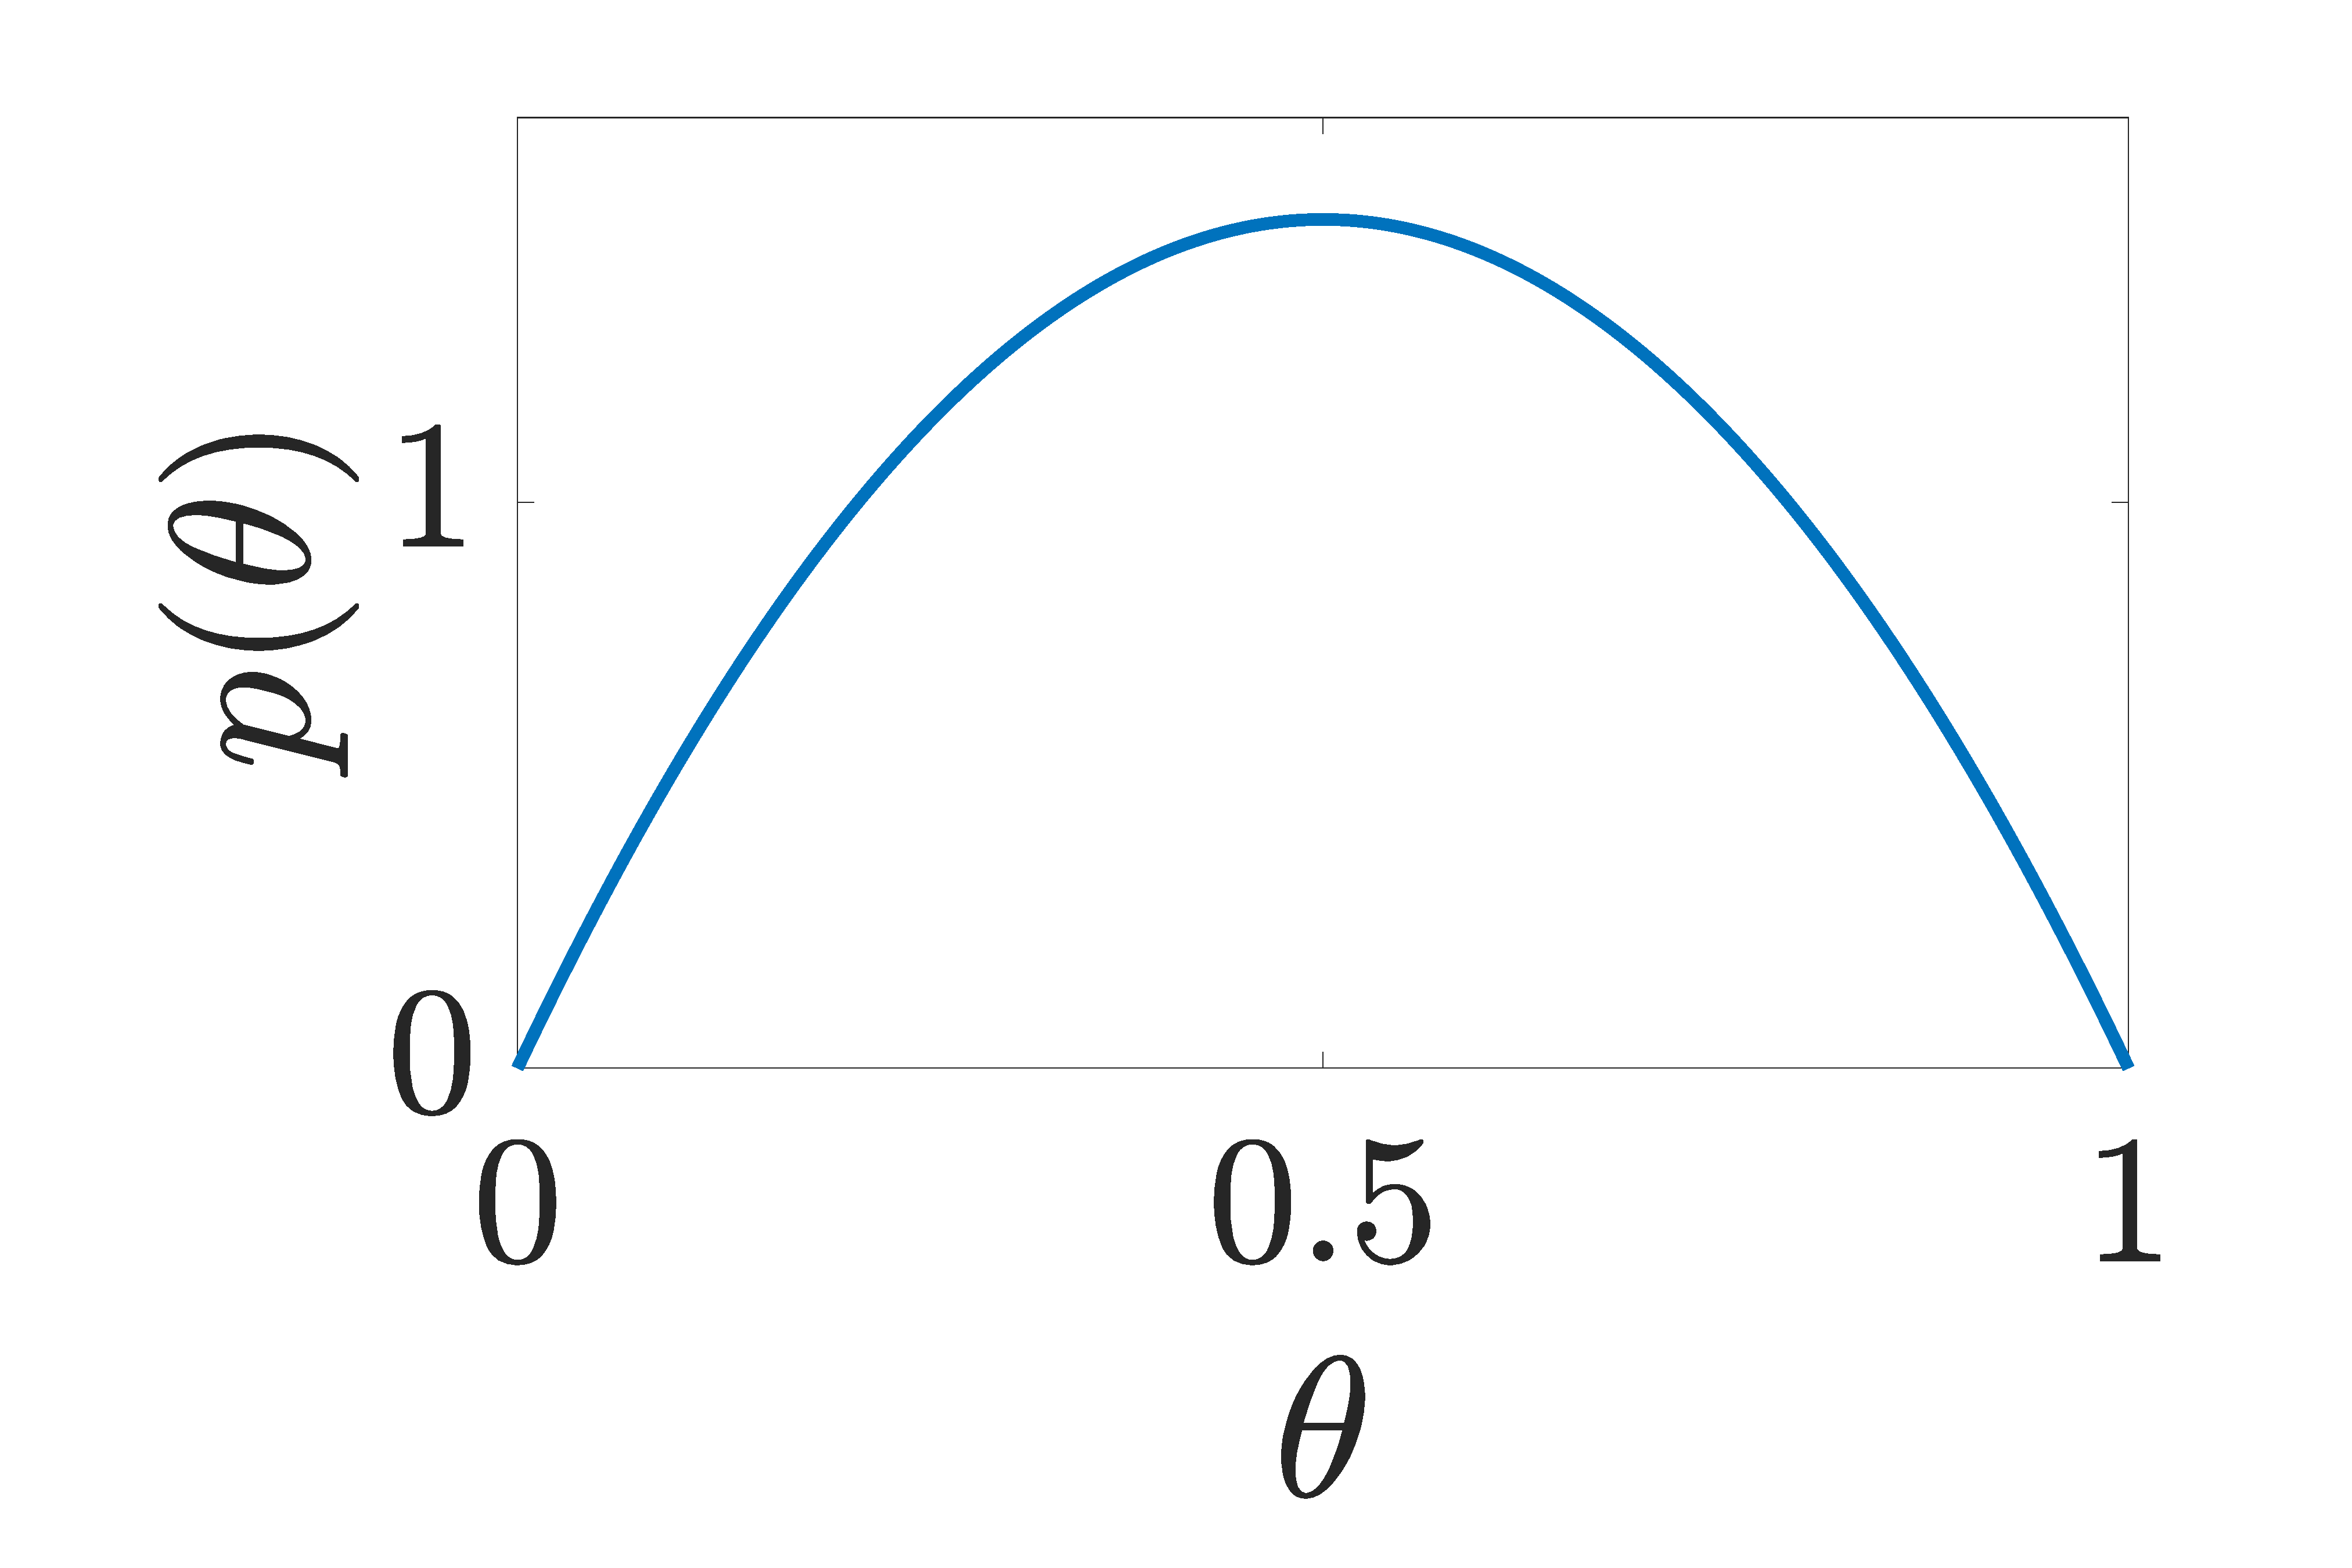
\includegraphics[width=\textwidth]{coin_flip_0}
		\caption{Prior \label{fig:inf:coin_flip:0}}
	\end{subfigure}
	\begin{subfigure}[t]{0.24\textwidth}
			\hspace{-10pt}
		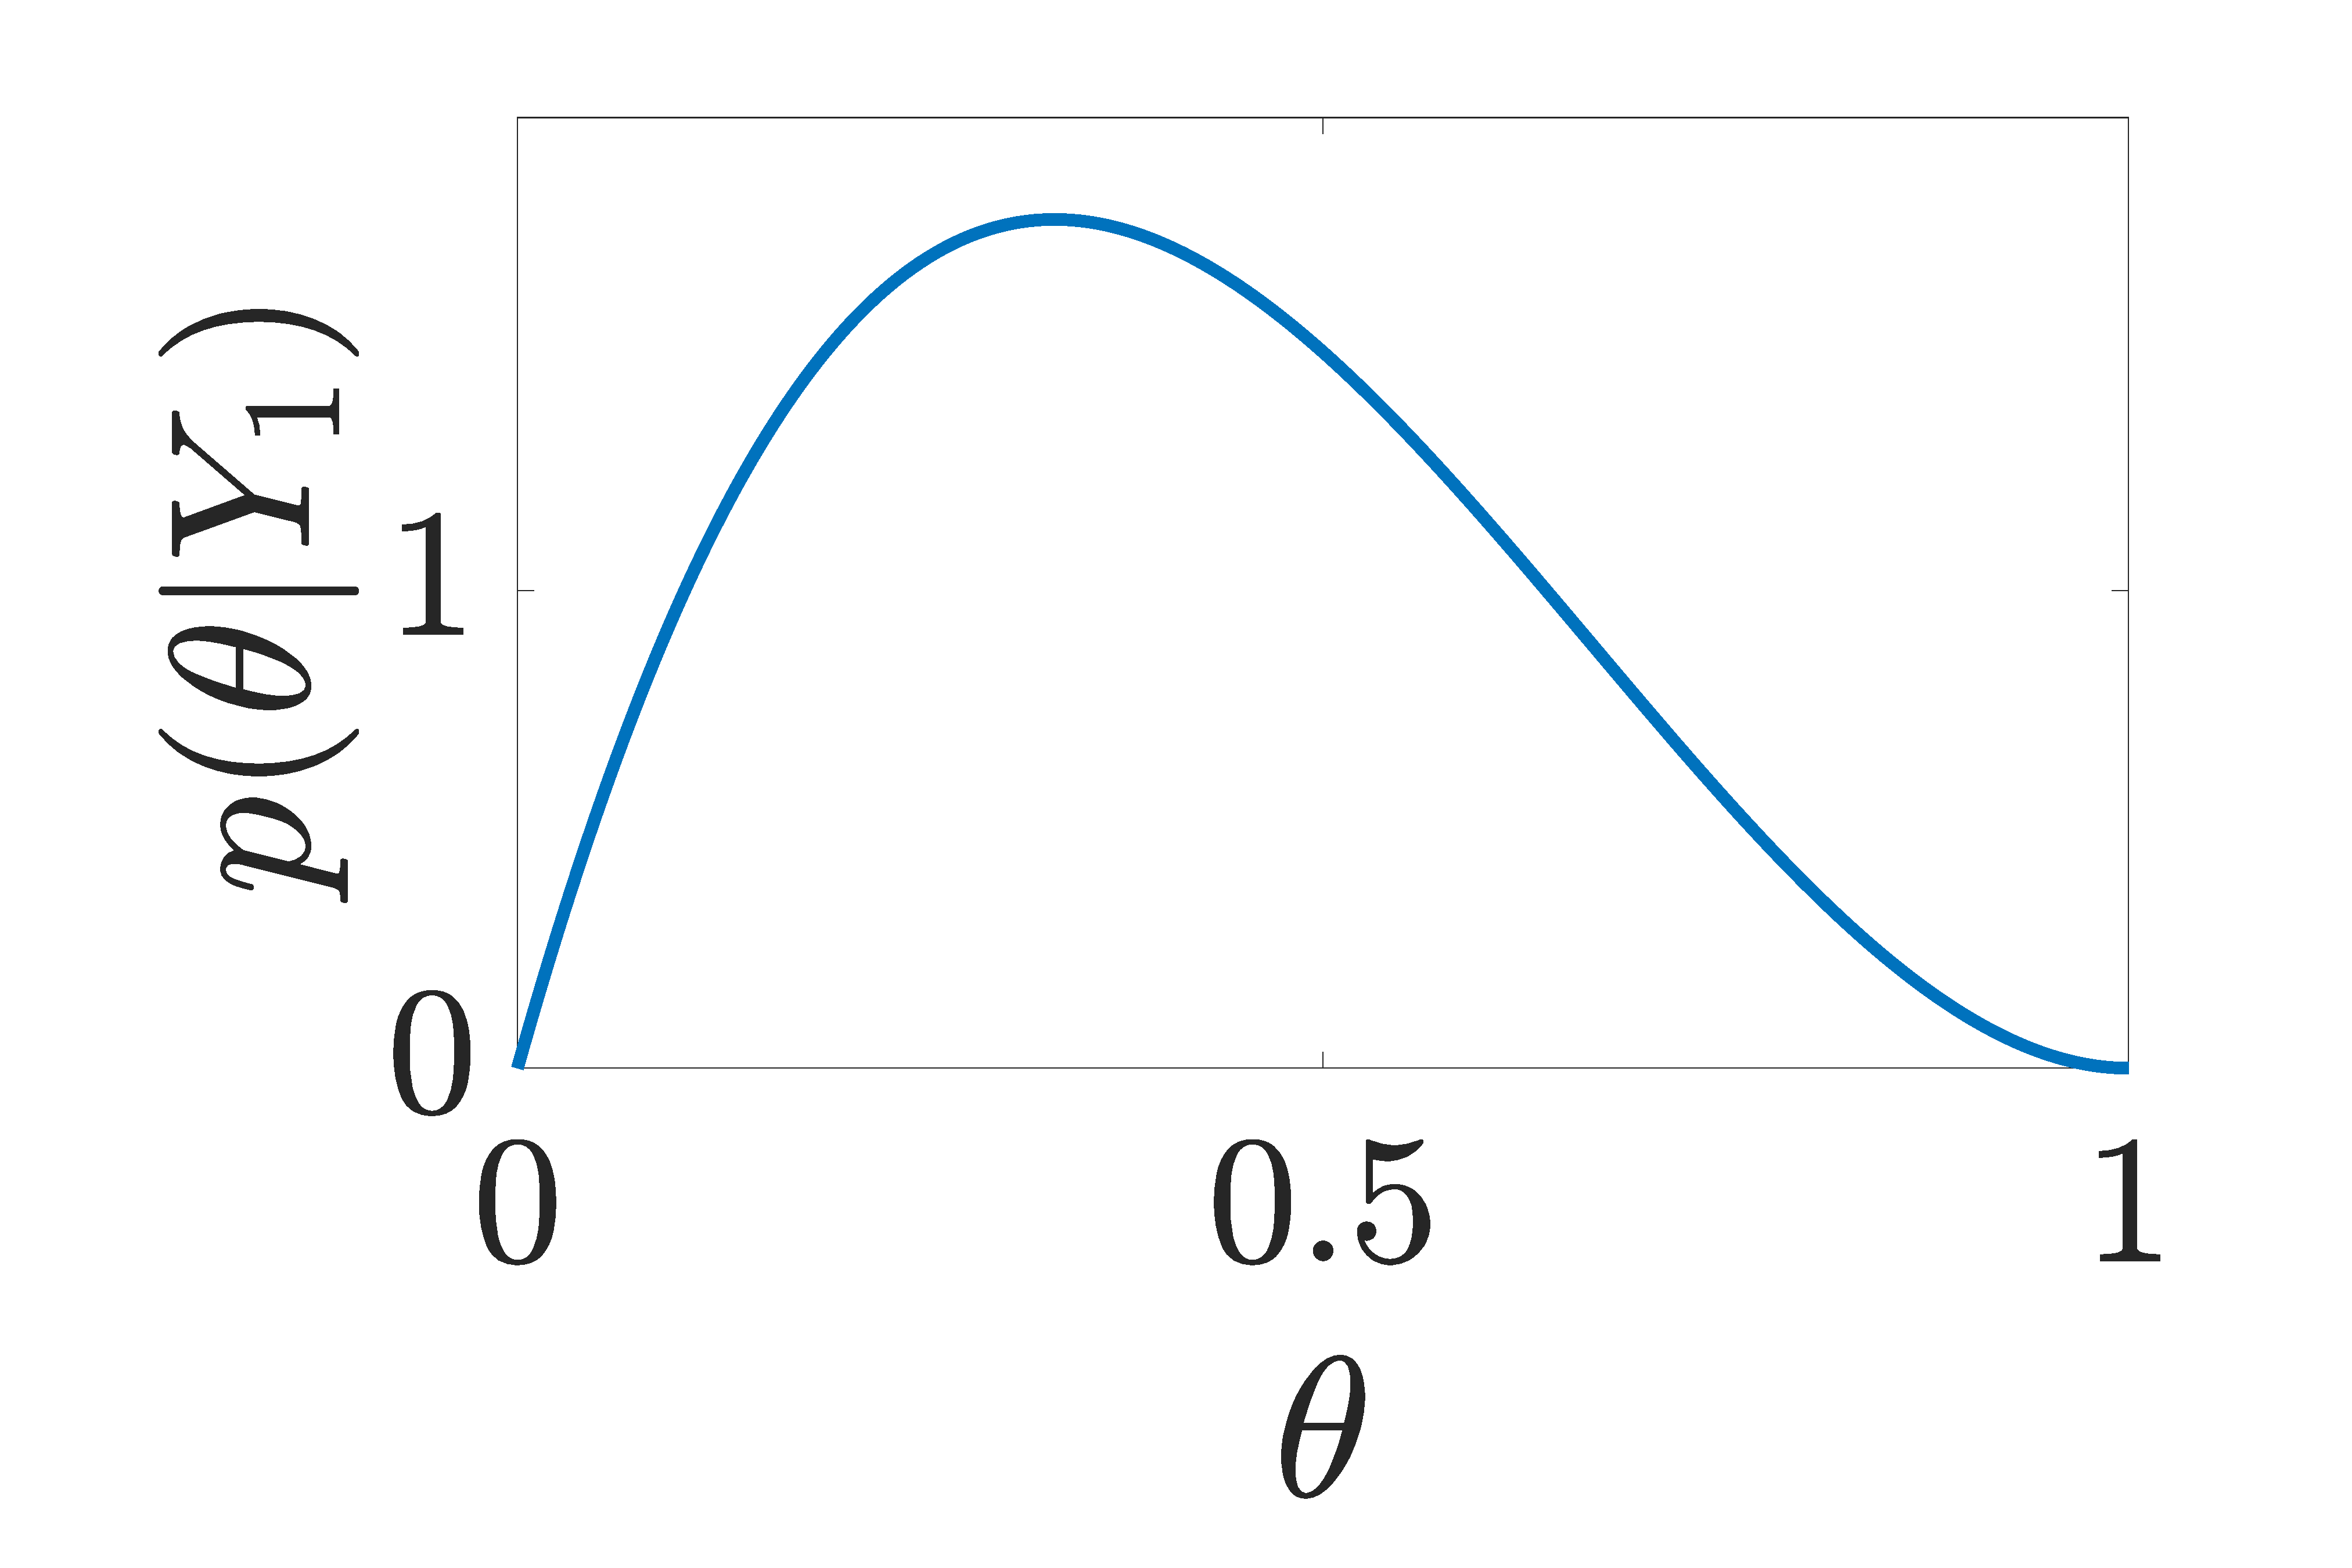
\includegraphics[width=\textwidth]{coin_flip_1}
		\caption{Posterior 1 flip \label{fig:inf:coin_flip:1}}
	\end{subfigure}
		\hspace{-3pt}
	\begin{subfigure}[t]{0.24\textwidth}
		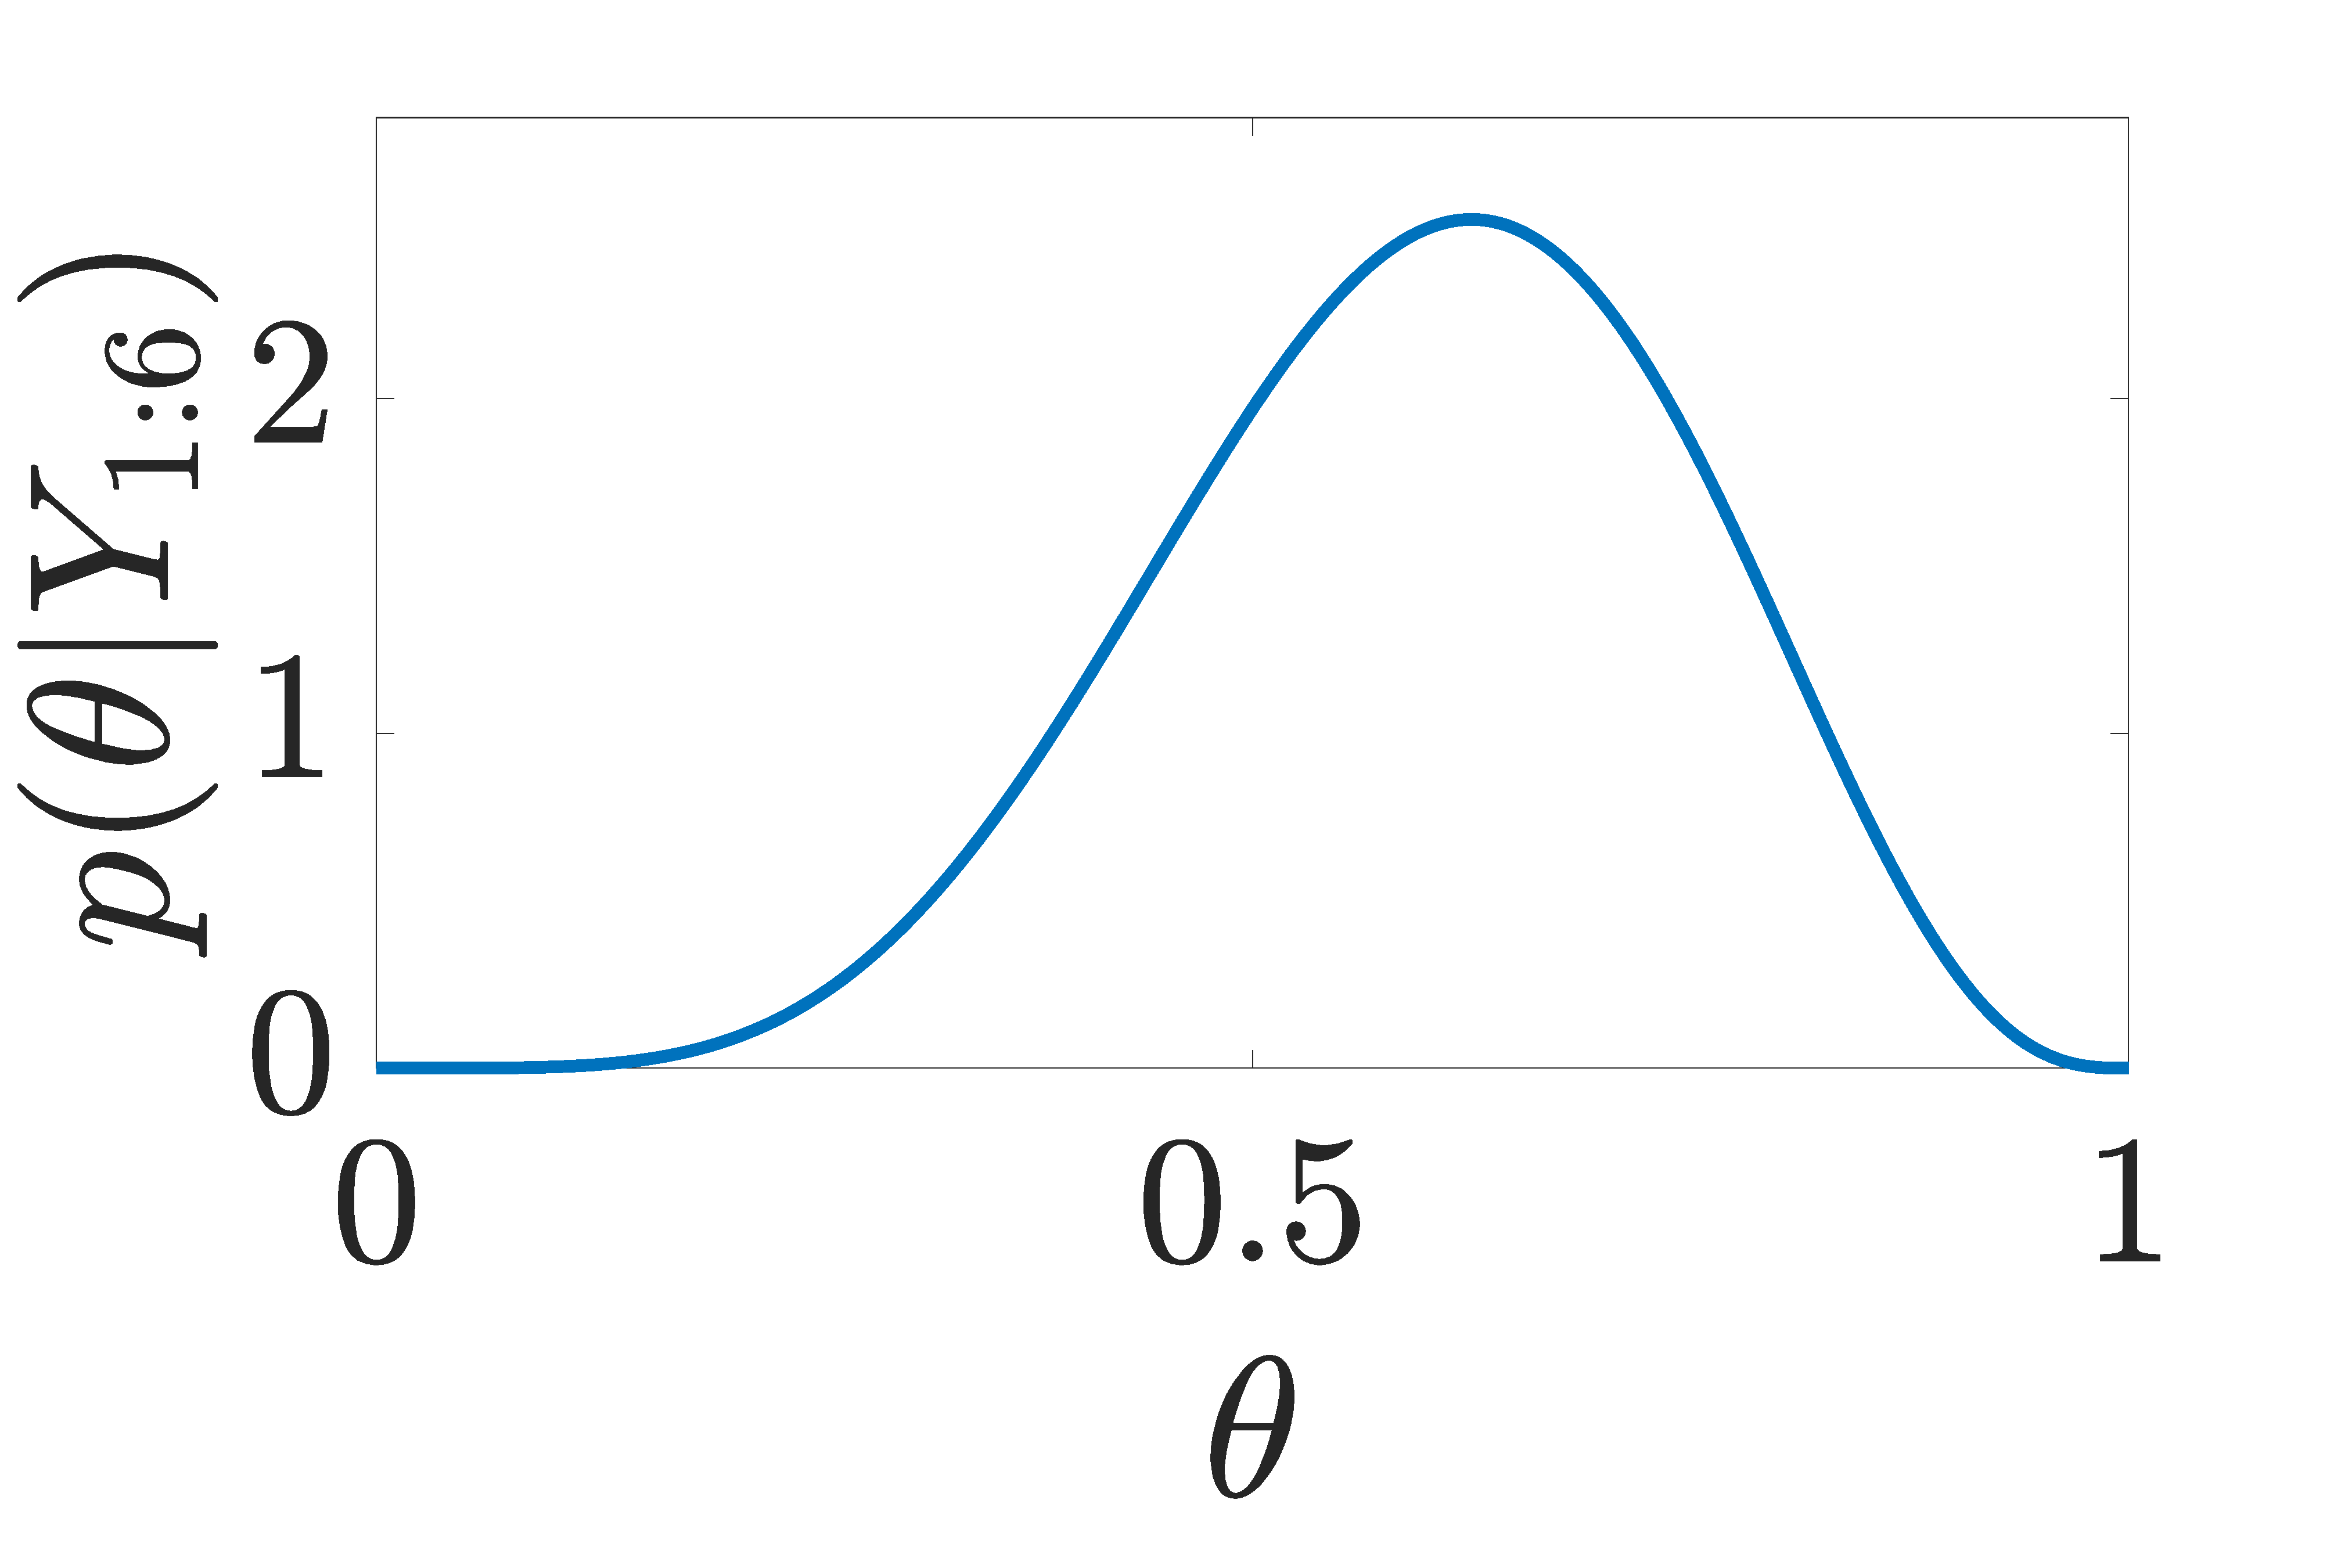
\includegraphics[width=\textwidth]{coin_flip_6}
		\caption{Posterior 6 flips \label{fig:inf:coin_flip:6}}
	\end{subfigure}
	\hspace{3pt}
	\begin{subfigure}[t]{0.24\textwidth}
		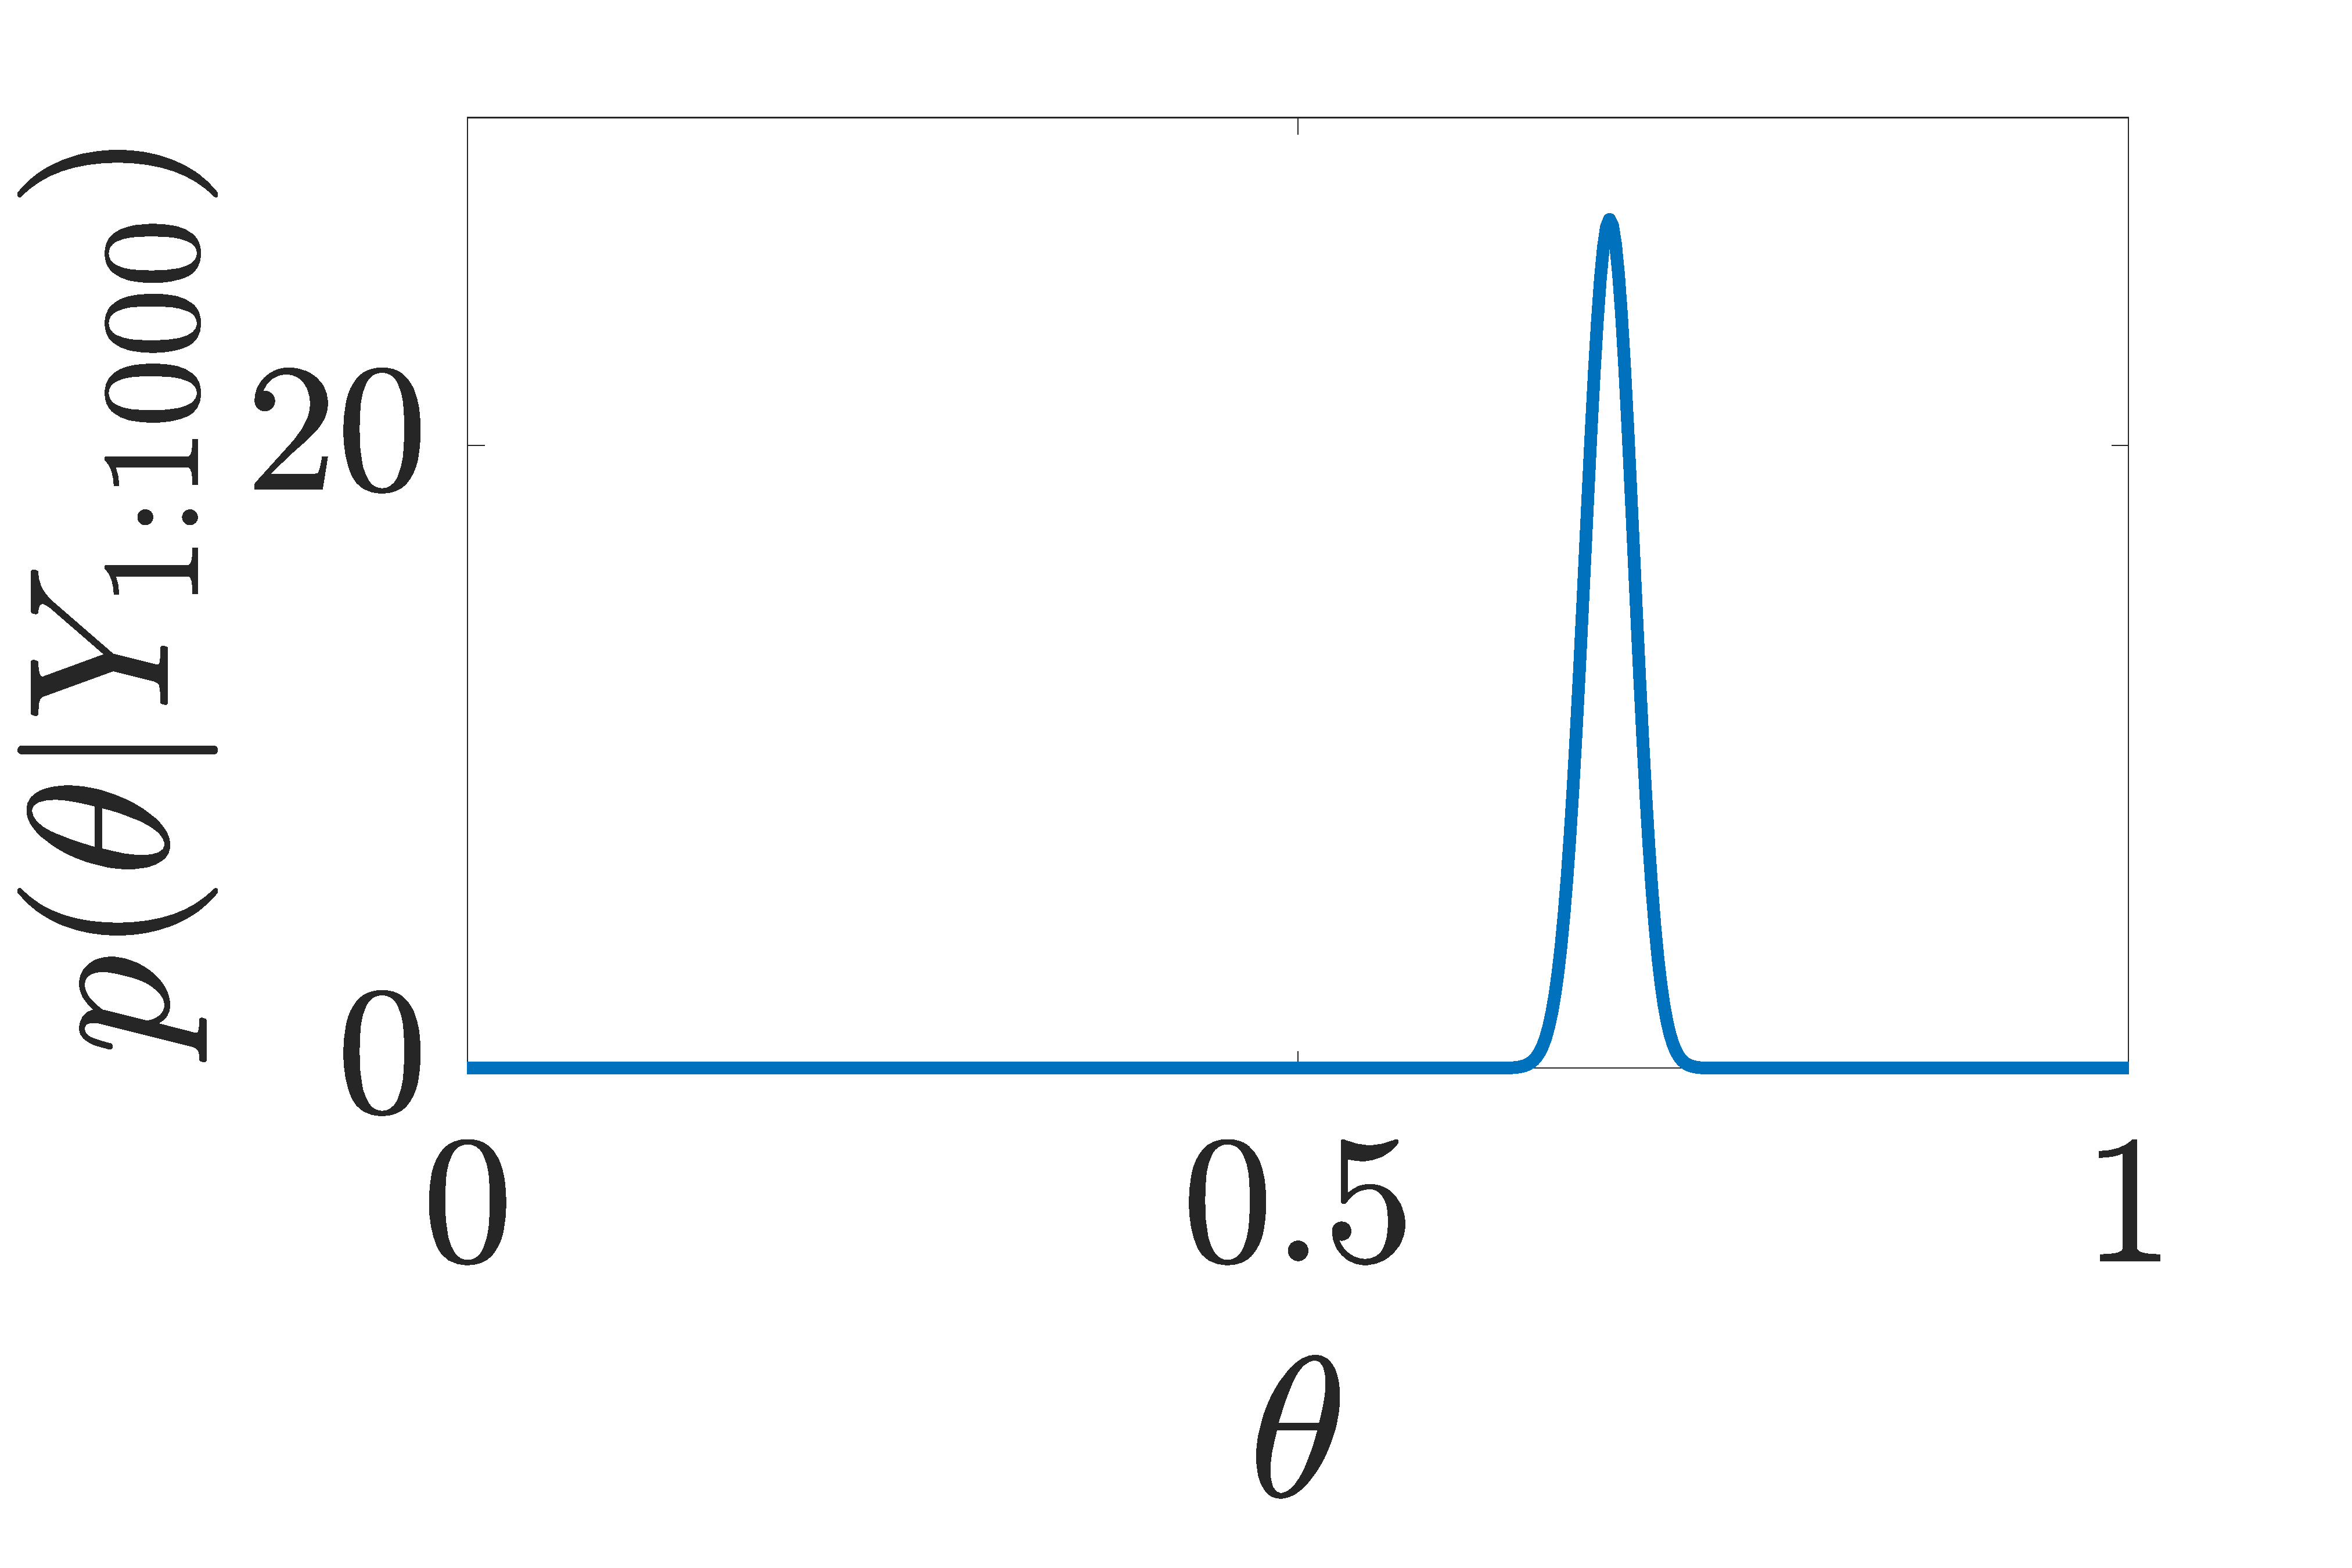
\includegraphics[width=\textwidth]{coin_flip_1000}
		\caption{Posterior 1000 flips \label{fig:inf:coin_flip:1000}}
	\end{subfigure}
	\caption{Prior and posteriors for coin flip example after different numbers
		of observations. \vspace{-5pt}
		\label{fig:inf:coin_flip}}
\end{figure}

If we now flip the coin again, our previous posterior~\eqref{eq:prob:beta_post_1} becomes our
prior and we can incorporate the new observations in the same way.  
Through our previous conjugacy result, then if we observe $n_{H}$ heads
and $n_{T}$ tails and our prior is $\textsc{Beta}(\theta ; \alpha, \beta)$ then our posterior is
$\textsc{Beta}(\theta ; \alpha+n_H, \beta+n_T)$.
Thus if our sequence of new
observations is $HTHHH$ then our new posterior is
\begin{align}
p(\theta | y_1,\dots,y_6) = \frac{p(y_2,\dots,y_6 | \theta)p(\theta | y_1)}
{\int p(y_2,\dots,y_6 | \theta)p(\theta | y_1) d\theta} = \textsc{Beta}\left(\theta ; 6,4\right),
\end{align}
which is shown in Figure~\ref{fig:inf:coin_flip:6}.  We see now that our belief for the probability of heads
has shifted higher and that the uncertainty has reduced because of the increased number
of observations.
After seeing a total of $1000$ observations as shown in Figure~\ref{fig:inf:coin_flip:1000}, we
find that the posterior has predominantly collapsed down to a small range of $\theta$.

Having calculated our posterior, we can now make
predictions using the \emph{posterior predictive distribution} which marginalizes out over
the parameters.  For the coin flip case, we have
\begin{align}
\label{eq:bayes:post-pred}
p( y_{N+1}=H | y_{1:N}) &= \int p(y_{N+1}=H, \theta | y_{1:N}) d\theta
= \int p(y_{N+1}=H | \theta) p(\theta | y_{1:N})  d\theta \nonumber \\
&= \int  \theta \; \textsc{Beta}(\theta ; \alpha+n_H, \beta+n_T) d\theta 
%= \int  
%\frac{\Gamma(\alpha+\beta)}{\Gamma (\alpha) \Gamma(\beta)} 
%\theta^{\alpha} (1-\theta)^{\beta-1} d\theta = 
%\frac{\Gamma(\alpha+\beta) \Gamma (\alpha+1)}{\Gamma (\alpha) \Gamma(\alpha+1+\beta)} \nonumber \\
=\frac{\alpha+n_H}{\alpha+n_H+\beta+n_T}
\end{align}
where we have used the known result for the mean of the Beta distribution.
The role of the parameters $\alpha$ and $\beta$ in our prior now become apparent
-- they take on the role of pseudo-observations.  Our prediction is in line with the
empirical average from seeing $\alpha+n_H$ heads and $\beta+n_T$ tails.  The larger
$\alpha+\beta$ is then the strong our prior compared to the observations, while we
can skew towards heads or tails being more likely by changing the relative values of $\alpha$
and $\beta$.

More generally the posterior predictive distribution will depend on a queried input point.
To demonstrate this, consider the example of a Bayesian linear regression from inputs $x\in\real^D$
to outputs $y\in\real$.  Assume that we have $N$ observations $\mathcal{D} = \{x_n,y_n\}_{n=1}^N$
and let $\mathbf{x}=[x_1,\dots,x_N]^T$ and $\mathbf{y}=[y_1,\dots,y_N]^T$ respectively be 
a $N\times D$ matrix and a column vector whose rows correspond to the different data points.
Our regression is of the form $y_n= x_n^T\mathbf{w}+b+\epsilon_n$ where $\mathbf{w}\in\real^D$, $b\in\real$
and each $\epsilon_n \iid \mathcal{N}(0,\sigma^2)$.  This implies a likelihood of
\begin{align}
\label{eq:bayes:linear-reg-lik}
p(\mathbf{y}|\mathbf{x},\mathbf{w},b,\sigma) = \prod_{n=1}^{N} p(y_n | x_n, \mathbf{w}, b, \sigma) = 
\prod_{n=1}^{N} \mathcal{N}(y_n;x_n^T\mathbf{w}+b,\sigma^2).
\end{align}
For simplicity, we will assume that $\sigma$ and $b$ are known fixed parameters,
but we will put a prior on $\mathbf{w}$, namely $p(\mathbf{w}) = \mathcal{N}(\mathbf{w};\mathbf{0},C)$
where $C$ is a fixed covariance matrix, in order to perform inference.
%% and $s$ a fixed scalar standard deviation.
%We further assume that $p(\mathbf{w},b | \sigma) = p(\mathbf{w}) p(b) $, i.e. that all
%three parameters are independent under the prior.
To make predictions, we first calculate the posterior
\begin{align}
p(\mathbf{w}| \mathcal{D}, b,\sigma) &= \mathcal{N}(\mathbf{w};\mathbf{0},C)
\prod_{n=1}^{N} \mathcal{N}(y_n;x_n^T \mathbf{w}+b,\sigma^2) = \mathcal{N}\left(\mathbf{w} ; m, S\right) \\
\mathrm{where} \quad m &= S^{-1} \mathbf{x}^T \left(\mathbf{y}-b\right)/\sigma^2 \quad
\mathrm{and} \quad S = \left( C^{-1}+\frac{\mathbf{x}^T\mathbf{x}}{\sigma^2}\right)^{-1}. \nonumber
%&= \mathcal{N}\left(\mathbf{w} ; \left( C^{-1}+\frac{\mathbf{x}^T\mathbf{x}}{\sigma^2}\right)^{-1} 
%\frac{\mathbf{x}^T \left(\mathbf{y}-b\right)}{\sigma^2},
%\left( C^{-1}+\frac{\mathbf{x}^T\mathbf{x}}{\sigma^2}\right)^{-1} \right),
\end{align}
We have omitted the necessary linear algebra (see for example~\cite{bishop2006pattern}
Sections 2.3.3 and 3.3)
but note the conjugacy between
the normal distribution and itself.  Prediction now uses the posterior predictive, marginalizing
over the parameters in the same manner as the coin flip example.  Here though, we are interested
in predicting the output $\tilde{y}$ at a particular input point $\tilde{x}$ for which we have
\begin{align}
p(\tilde{y}| \tilde{x},\mathcal{D}, b,\sigma) &= \int p(\tilde{y}| \tilde{x},\mathbf{w}) 
p(\mathbf{w}| \mathcal{D}, b,\sigma) d\mathbf{w} 
= \int \mathcal{N}(\tilde{y};\tilde{x}^T\mathbf{w}+b,\sigma^2)
\mathcal{N}\left(\mathbf{w} ; m, S\right) d\mathbf{w} \nonumber \\
&= \mathcal{N} \left(\tilde{y} \; ; \;\tilde{x}^Tm+b, \; \tilde{x}^T S^{-1}\tilde{x}+\frac{1}{\sigma^2} \right)
\end{align}
which again follows from standard results for Gaussian distributions.  We, therefore, have
an analytic predictive distribution at any possible input point.
Though this linear regression example might seem overly simple for practical purposes, we
will see in Section~\ref{sec:opt:GPs} that substantially more advanced models, such as
Gaussian processes, can be viewed as linear regressions between a set of features on the inputs $\phi(x)$
and the output $y$.

The models we have introduced so far are specific examples of Bayesian modeling and will
clearly only be applicable or appropriate in very particular scenarios.  
%However, the only restrictions we
%have in order to carry out Bayesian modeling is that the prior and likelihood are valid probability distributions
%(in practice even these requirements can often be relaxed).  
Bayesian modeling is at its heart a
generative approach and its real power will be when we design a rich and expressive \emph{generative model} 
that reflects our application-specific knowledge.  In other words, we can define our model
by carefully constructing a stochastic process that describes how the parameters  and data are generated.  For
our object recognition example at the start of the section, this would correspond to a graphics generator for
sampling scenes.
More generally, the model corresponds to the joint distribution on parameters and data $p(\theta,\mathcal{D})$.
We can then think of observing real data as refining our model through \emph{conditioning}, providing an updated distribution
on the parameters $p(\theta|\mathcal{D})$ and subsequent predictions that incorporate the information from the data.  The more
flexible we make our generative model, the more we can make it represent the data.  The less flexible
we make the generative model, the more weighting is given to our prior assumptions.

We finish by making a technical point of note about the behavior of Bayesian methods in the limit of large
data.  Assume that our likelihood model $p(\mathcal{D}|\theta)$ is correct such that the data $\mathcal{D} = y_{1:N}$
is generated according to 
$p(y_{1:N} | \theta^*)$ where $\theta^*$ are the (finite) set of ground truth parameters 
and the prior $p(\theta)$ satisfies $p(\theta^*)>0$.  Informally speaking, the Bernstein-Von Mises theorem now states
that in the limit of large $N$, the posterior distribution $p(\theta | y_{1:N})$ converges to a normal distribution 
with mean $\theta^*$ and variance of order $O(1/N)$ 
(i.e. it decreases at a rate $1/N$)~\citep{doob1949application,freedman1963asymptotic}.  This is a hugely important
result in Bayesian statistics as it demonstrates that, when our model assumptions are correct, we converge to the true parameters 
and the posterior becomes independent of the prior when we are provided with sufficient data.  It further transpires that when no such $\theta^*$ exists (i.e. our model is misspecified), the convergence
is instead to the parameters $\hat{\theta}$ which minimize the Kullback-Leibler (KL) divergence\footnote{The KL divergence
	can informally be thought of as a measure of discrepancy between two distributions.  Though
	it is not symmetric in its inputs, it is always non-negative and zero if and only if the two distributions are the same.} to the true data generating
distribution $p^*(y_{1:N})$, namely
\begin{align}
\hat{\theta} = \argmin_{\theta} \textsc{KL}\left(p^*(y_{1:N}) \| p(y_{1:N} | \theta)\right)
= \argmin_{\theta} \int p^*(y_{1:N}) \log \left(\frac{p^*(y_{1:N})}{p(y_{1:N}|\theta)}\right) dy_{1:N}.
\end{align}
See for example~\citep{kleijn2012bernstein} and the references therein for further details.
% !TEX root = ../main.tex

\section{Graphical Models}
\label{sec:bayes:paradigm:graph}

Generative models will typically have many variables and a complex \emph{dependency structure}.
In other words, many of variables will be conditionally independent of one another given values for
other variables.  Graphical models are a ubiquitously used method for representing and reasoning
about generative models with a particular focus on the dependency structure.  At a high-level, they
capture how the joint probability distribution can be broken down into a product of different factors, 
each defined over
a subset of the variables.  They are formed of a number of connected nodes, where each node
represents a random variable in the model and each variable has its own node.  Links between nodes in
the model represent dependencies: any two connected nodes have an explicit dependency.
Various independence assumptions can be deduced from the graphical model, though the exact nature
of these deductions will depend on the type of graphical model -- nodes without direct links
between them will often still be dependent.

Graphical models can be separated into two distinct classes: directed graphical
models and undirected graphical models.  Undirected graphical models, also known as Markov random
fields, imply no ordering on their factorization and are used only to express conditional independences
between variables.  They are used in scenarios where it is difficult to specify the target distribution in a
structured generative way, e.g. in Boltzmann machines~\citep{ackley1985learning}.  To give 
a more concrete example, if modeling whether it will rain at various locations then there
is a clear dependence between nearby locations, but not a natural ordering to the joint probability
distribution of where it will rain.   Independence in undirected graphical models can be deduced
through the \emph{global Markov property} which states that any two non-intersecting subsets of the 
variables $A$ and $B$ are
conditionally independent given a third, separating, subset $C$ if there is no path between $A$ and
$B$ that does not pass through $C$.  This means, for example, that each variable is conditionally
independent of all the other variables given its neighbors.

Our main focus, though, will instead be on directed graphical models and in particular directed acyclic 
graphical models (DAGs), i.e. directed graphical models containing no cycles or loops one can follow 
and arrive back in the starting position.  DAGs, also known as Bayesian networks, are particularly
useful in the context of Bayesian modeling because they can be used to express \emph{casual relationships}.
As such, they can be used as a piecewise explanation for how the joint distribution is generated.
Not only does this form a natural means to describe and design models in the first place, 
we can carefully order the breakdown to factorize the distribution into only terms we know.  For example,
in the linear regression model, we did not know (at least when the model was first defined) 
$p(\mathcal{D})$ but we did know $p(\mathbf{w})$ and $p(\mathcal{D} | \mathbf{w})$.  Therefore even
though we could factorize our joint $p(\mathcal{D}, \mathbf{w})$ as 
$p(\mathbf{w} | \mathcal{D})p(\mathcal{D})$ and construct a DAG this way, it is much more convenient
to factorize and construct the DAG the other way round, namely as 
$p(\mathcal{D} | \mathbf{w})p(\mathbf{w})$.
We will generally not have access to all possible factorizations
in an analytic form as otherwise there would be no need to perform inference.
As a rule-of-thumb, when we define a model using a DAG, we need to be able to define the 
probability of each variable given its \emph{parents}, i.e. all the nodes with links from that node
towards the node the question.

The demonstrate this factorization more explicitly and give a concrete example of a DAG, consider a joint model
$p(a,b,c)$.  By the product rule, we can break down this joint distribution into a number of different
factorizations, but some will typically be more useful than others.  Imagine a medical diagnostic
example where $a$ represents lifestyle and genetic factors of a patient such as whether they smoke
or have unknown preexisting conditions, 
$b$ represents the presence of lung cancer, and $c$ represents symptoms 
such as a persistent cough.  Here we have the following natural breakdown of the joint distribution
\begin{align}
\label{eq:bayes:example-graph}
p(a,b,c) = p(a) p(b|a) p(c|a,b).
\end{align}
\begin{wrapfigure}{r}{0.35\textwidth}
	\vspace{-12pt}
	\centering 
	\resizebox{.32\textwidth}{!}{
		% !TEX root = ../../main.tex

\begin{tikzpicture}

\node[obs]                               (c) {$c$};
\node[latent, above=of c, xshift=-1.2cm] (a) {$a$};
\node[latent, above=of c, xshift=1.2cm]  (b) {$b$};

\edge {a,b} {c} ; %
\edge {a} {b} ; %

\end{tikzpicture}
	}
	\caption{Simple example DAG corresponding to~\eqref{eq:bayes:example-graph}
		\label{fig:bayes:simple-graph}}
	\vspace{-10pt}
\end{wrapfigure}
The lifestyle and genetic factors will generally either be known or can be estimated from tests or
simply prevalence within the population.  Given these factors, the likelihood of somebody developing
lung cancer can be modeled using existing data and domain expertise.   Given the lifestyle and
genetic factors and the knowledge of whether lung cancer is present, we can predict what
symptoms might be observed.  We can express our model and this factorization using
the DAG shown in Figure~\ref{fig:bayes:simple-graph}.
  Here we have shaded in $c$ to express the fact that this is
observed.  The graphical model expresses our dependency structure as we have the probability
of each node given its parents.  As shown in~\eqref{eq:bayes:example-graph}, the product of
all these factors is equal to our joint distribution.  The DAG has thus formed a convenient means
of representing our generative process.

Clearly, our aim for this problem will be to find the probability cancer is present given
the symptom, i.e. $p(b|c)$, which will
require Bayesian inference.
An important feature of the breakdown of graphical models will become apparent when we
consider how we can conduct such inference for more a general class of 
models where the solution is not analytic in Chapter~\ref{chp:inf}.  Here knowing the dependency
structure and, in particular, the independence relationships, will be essential to many inference 
schemes such as message passing schemes.

A natural question is now how can we deduce the independence relationships from a DAG?
This can be done by introducing the notion of \emph{d-separation}~\citep{pearl2014probabilistic}.
Consider three arbitrary, non-intersecting, subsets $A$, $B$, and $C$ of our DAG.  $A$ and $B$
are conditionally independent given $C$ if there are no \emph{unblocked} paths from $A$ to $B$
(or equivalently from $B$ to $A$), in which case $A$ is said to be d-separated from $B$ by $C$.  
Paths do not need to be in the directions defined by the DAG but are blocked if either
\begin{enumerate}
		\setlength\itemsep{-0.1em}
	\item Consecutive arrows both point towards a node that is not in and
	has no descendants in $C$, i.e. we cannot get to any of the nodes in $C$ by following the arrows
	from this node.
	\item Consecutive arrows meet at a node in $C$ and one of them
	points away from the node.
\end{enumerate}
Note that only the first of these rules is necessary for establishing marginal independence
between nodes as this rule can still be used when $C$ is empty.
Examples of blocked paths are shown in Figure~\ref{fig:bayes:blocked-graphs} while examples of unblocked paths
are shown in Figure~\ref{fig:bayes:unblocked-graphs}, explanations for which are given in the captions.
For a more comprehensive introduction to establishing independence in DAGs, we
refer the reader to Section 8.2 of~\cite{bishop2006pattern}.

\begin{figure}[t]
	\centering 
	\begin{subfigure}[t]{0.32\textwidth}
		\centering
		\resizebox{0.9\textwidth}{!}{
		% !TEX root = ../../main.tex

\begin{tikzpicture}

\node[obs]                               (c) {$c$};
\node[latent, above=of c, xshift=-1.2cm] (a) {$a$};
\node[latent, above=of c, xshift=1.2cm]  (b) {$b$};

\edge {a} {c} ; %
\edge {c} {b} ; %

\end{tikzpicture}}
		\caption{\label{fig:bayes:block1}}
	\end{subfigure}
	\begin{subfigure}[t]{0.32\textwidth}
		\centering
		\resizebox{0.9\textwidth}{!}{
		% !TEX root = ../../main.tex

\begin{tikzpicture}

\node[obs]                               (c) {$c$};
\node[latent, below=of c, xshift=-1.2cm] (a) {$a$};
\node[latent, below=of c, xshift=1.2cm]  (b) {$b$};

\edge {c} {a} ; %
\edge {c} {b} ; %

\end{tikzpicture}}
		\caption{\label{fig:bayes:block2}}
	\end{subfigure}
	\begin{subfigure}[t]{0.32\textwidth}
		\centering
		\resizebox{0.9\textwidth}{!}{
		% !TEX root = ../../main.tex

\begin{tikzpicture}

%\node[latent]  (a) {$a$};
%\node[latent, right=2.4cm of a]  (b) {$b$};
%\node[latent, below= of a, xshift=1.2cm] (d) {$d$};
%%\node[latent, right=1.8cm of d]             (e) {$e$};
%
%%\edge {d} {e} ; %
%\edge {a} {d} ; %
%\edge {b} {d} ; %

\node[latent]                               (d) {$d$};
\node[latent, above=of d, xshift=-1.2cm] (a) {$a$};
\node[latent, above=of d, xshift=1.2cm]  (b) {$b$};

\edge {a} {d} ; %
\edge {b} {d} ; %

\end{tikzpicture}}
		\caption{\label{fig:bayes:block3}}
	\end{subfigure}
	\caption{Examples of DAGs blocked between $a$ and $b$.  \textbf{(a)} is blocked
		by the second rule of d-separation.  More specifically we have 
		$p(b|a,c)=\frac{p(a,b,c)}{p(a,c)} = \frac{p(a)p(c|a)p(b|c)}{p(a)p(c|a)} = p(b|c)$.
		\textbf{(b)} is blocked by the first rule of d-separation.  Here we have
		$p(b|a,c)=\frac{p(c)p(a|c)p(b|c)}{p(c)p(a|c)} = p(b|c)$.  Consequently, for \textbf{(a)} 
		and \textbf{(b)} then $a$ and $b$ are conditionally independent given $c$ .
		\textbf{(c)} is an instead example of where $a$ and $b$ are \emph{marginally} independent.  Here
		the path between $a$ and $b$ is blocked because the the arrows meet head-to-head at 
		$d$ and neither $d$ nor any of its
		descendants are observed.  We thus have $p(b|a) = \frac{p(a)p(b)p(d|a,b)}{p(a)p(d|a,b)} = p(b)$.
		Note though that $a$ and $b$ are note conditionally independent given $d$ as
		the path becomes unblocked if this is observed (see Figure~\ref{fig:bayes:unblocked-graphs}).
		\label{fig:bayes:blocked-graphs}}
\end{figure}

\begin{figure}[t]
	\centering 
	\hspace{-15pt}
	\begin{subfigure}[t]{0.32\textwidth}
		\centering
		\resizebox{0.9\textwidth}{!}{
		% !TEX root = ../../main.tex

\begin{tikzpicture}

\node[latent]                               (d) {$d$};
\node[latent, above=of d, xshift=-1.2cm] (a) {$a$};
\node[latent, above=of d, xshift=1.2cm]  (b) {$b$};

\edge {a} {d} ; %
\edge {d} {b} ; %

\end{tikzpicture}}
		\caption{\label{fig:bayes:unblock1}}
	\end{subfigure}
	\begin{subfigure}[t]{0.32\textwidth}
		\centering
		\resizebox{0.9\textwidth}{!}{
		% !TEX root = ../../main.tex

\begin{tikzpicture}

\node[latent]                               (d) {$d$};
\node[latent, below=of d, xshift=-1.2cm] (a) {$a$};
\node[latent, below=of d, xshift=1.2cm]  (b) {$b$};

\edge {d} {a} ; %
\edge {d} {b} ; %

\end{tikzpicture}}
		\caption{\label{fig:bayes:unblock2}}
	\end{subfigure}
	\begin{subfigure}[t]{0.32\textwidth}
		\centering
		\resizebox{1.1\textwidth}{!}{
		% !TEX root = ../../main.tex

\begin{tikzpicture}

\node[latent]                               (d) {$d$};
\node[latent, above=of d, xshift=-1.2cm] (a) {$a$};
\node[latent, above=of d, xshift=1.2cm]  (b) {$b$};
\node[obs, right=1.2cm of d]             (c) {$c$};

\edge {d} {c} ; %
\edge {a} {d} ; %
\edge {b} {d} ; %

\end{tikzpicture}}
		\caption{\label{fig:bayes:unblock3}}
	\end{subfigure}
	\caption{Examples of DAGs unblocked between $a$ and $b$. For \textbf{(a)} then the path from $a$ to
		$b$ is not blocked by the d-separation rules.  Perhaps more intuitively, we have that
		$p(b|a) = \int p(b,d|a) dd = \int p(b|d)p(d|a) dd \neq p(b)$ unless $p(d|a)=p(d)$.
		Similarly there is an unblocked path for \textbf{(b)} from $a$ to $b$ as the path
		that does not pass through any observed nodes or nodes with both arrows points towards it.
		Here we have $p(b|a) = \frac{p(d)p(a|d)p(b|d)}{p(a)p(d|a,b)} \neq p(b)$ again in general.
		The path in \textbf{(c)} is unblocked because of the phenomenon of \emph{explaining away}.
		The first rule of d-separation does not apply here because $c$ is an observed descendant of
		$d$.  We thus have that $a$ and $b$ are marginally independent as per Figure~\ref{fig:bayes:block3},
		but not conditionally independent given $c$ (and/or $d$). The rationale for explaining away can be thought
		of in terms of events needing an explanation -- if two precursor events (here $a$ and $b$) can give rise 
		to a third event (here $c$), then
		the third event occurring but not the first precursor event implies that the second precursor
		event occurs.  Thus the two precursor events are correlated because one \emph{explains away} the other.
		As described in Section~\ref{sec:prob:cond}, one example of this is that if a speed camera is
		triggered and the camera is not malfunctioning, this implies the vehicle is speeding, even though
		the vehicle speeding and the camera malfunctioning are marginally independent.	
		\label{fig:bayes:unblocked-graphs}}
\end{figure}

In the simple example of Figure~\ref{fig:bayes:simple-graph} there were no independence relationships and so
we gain little from working with the DAG compared to just the joint probability distribution.
A more advanced example where there are substantial independence relationships which can
be exploited is shown in Figure~\ref{fig:bayes:hmm}.
  This model is known as a hidden Markov 
model\footnote{The use of the tern HMM in the literature (and later in this paper) often also implies that
	the latent states are discrete variables, with the equivalent continuous model referred to as a
	(Markovian) state space model.} (HMM)
and has $T$ latent variables $x_{1:T}$ and $T$ observations $y_{1:T}$.  The joint distribution is as follows
\begin{align}
\label{eq:bayes:hmm}
p(x_{1:T},y_{1:T}) = p(x_1) p(y_1|x_1)\prod_{t=2}^{T} p(x_t|x_{t-1})p(y_t|x_t),
\end{align}
where each $x_t$ is
independent of $x_{1:{t-2}}$ and $y_{1:t-1}$ given $x_{t-1}$ and of $x_{t+2:T}$ and $y_{{t+1}:T}$ given $x_{t+1}$.
This is known as the Markov property and means that each latent variable only depends on the other
variables and observations through its immediate neighboring states.  In essence, the model has no memory as information
is passed forwards (or backwards) only through the value of the previous (or next) latent state.  A number of stochastic
processes and dynamical systems obey the Markov property and HMMs and their extensions are extensively used for
a number of tasks involving sequential data, such as DNA sequencing~\citep{durbin1998biological} and tracking
animals~\citep{dhir2016tracking,dhir2017interpreting} to name but a few. 
%For example, in a dynamical system, then the next state
%depends only on the dynamics of the system and its  current state (e.g. position velocity etc).

A key part of the appeal of HMMs is that the structure of the
DAG can be exploited to give analytic solutions to the resulting Bayesian inference whenever each $p(y_t | x_t)$ 
and $p(x_t | x_{t-1})$ is either a discrete or Gaussian distribution. Even when this does not hold, there 
are still a number of features of the dependency structure that can make the inference substantially easier.
As we will show in Chapter~\ref{chp:inf}, Bayesian inference is generally a challenging problem, often prohibitively so.
Therefore the (fast) analytic inference for HMMs is highly convenient.  However, it can mean that HMMs are perhaps overused.
More generally, simplifying approximations or unjustified assumptions are often made by Bayesian practitioners 
for tractability, e.g. by using an off-the-shelf model like an HMM with known analytic solution. Though often necessary, 
this must be done with extreme care and the implications of the approximations should carefully considered.  Unfortunately, 
quantifying the implications of approximations can be very difficult, given that they are typically made in the interest
of tractability in the first place.  The is a serious practical weakness of Bayesian modeling and should be factored 
into the decision processes of whether taking a Bayesian approach or not.  
%While taking a Bayesian approach for large projects, 
%one should, in general, avoid making approximations or non-clearcut assumptions until absolutely necessary, but also 
%keep in mind that it may be necessary to do so further down the line and account for this appropriately.

\begin{figure}[t]
	\centering 
	% !TEX root = ../../main.tex

\begin{tikzpicture}

\node[latent, minimum size=27pt] (x1) {$x_1$};
\node[latent, right=1.4cm of x1, minimum size=27pt] (x2) {$x_2$};
\node[right=1.4cm of x2] (x3) {{\tiny $\bullet \; \bullet \; \bullet$}};
\node[latent, right=1.4cm of x3, minimum size=27pt] (x4) {$x_{T\text{-}1}$};
\node[latent, right=1.4cm of x4, minimum size=27pt] (xT) {$x_T$};

\node[obs, below=of x1, minimum size=27pt] (y1) {$y_1$};
\node[obs, below=of x2, minimum size=27pt] (y2) {$y_2$};
%\node[obs, below=of x3] (y3) {$y_3$};
\node[obs, below=of x4, minimum size=27pt] (y4) {$y_{T\text{-}1}$};
\node[obs, below=of xT, minimum size=27pt] (yT) {$y_T$};

%\node[latent, above=of x1, xshift=-1.2cm, minimum size=27pt] (t) {$\theta$};

\edge {x1} {x2,y1} ; %
\edge {x2} {x3,y2} ; %
\edge {x3} {x4} ; %
\edge {x4} {xT,y4} ; %
\edge {xT} {yT} ; %

%\edge {t} {x1,x2};
%\edge[bend left=0] {t} {x4};
%\edge[bend left=10] {t} {xT};

\end{tikzpicture}
	\caption{DAG for a hidden Markov model.
		\label{fig:bayes:hmm}}
\end{figure}
% !TEX root = ../main.tex

\section{Frequentist vs Bayesian -- an Atheist's View on Two Religions}
\label{sec:bayes:religions}

We have just introduced the Bayesian approach to generative modeling, but this is far from
the only possible approach.  In this section, we will briefly introduce the alternative, \emph{frequentist},
approach.
  Unfortunately, there is often a substantial, and sometimes acrimonious, divide between those
who advocate Bayesian or frequentist methods within the statistics and machine learning communities.  Many people
have very strong views one way or another in the debate and it is easy, certainly as a graduate student,
to be sufficiently isolated on one side of the divide to completely detract oneself from the considerations of the
other.  It sometimes feels that the beliefs of some advocates of each side are so deep-rooted and 
fundamental that this almost a religious, rather than scientific divide.  Given the fierceness of the debate,
the actual statistical differences between the approaches (rather than the well-known philosophical differences we touched
on in Section~\ref{sec:prob:prob} which are often dubiously used for justification) are often surprisingly poorly understood.
Our aim in this section is not to advocate the use of one approach over the other, but to (hopefully objectively)
highlight these statistical differences and demonstrate that \emph{both} approaches have flaws, such that ``head in the sand''
mentalities either way can be highly detrimental.  
We note that whereas Bayesian methods are always, at least in theory, generative~\citep[Section~14.1]{gelman2014bayesian},
frequentist methods can be either generative or discriminative. 
As we have already discussed differences between generative and
discriminative modeling in Section~\ref{sec:bayes:discrim} we will omit this difference from our subsequent discussion.

At their root, the difference between Bayesian and frequentist methods stem from distinct fundamental
assumptions: frequentist modeling presumes fixed parameters, Bayesian modeling assumes fixed data.  In many ways,
both of these assumptions are actually quite silly. Why assume fixed parameters when we do not have enough
information about from the data to be certain of the correct value?  Why ignore that fact that other data could have 
been generated by the underlying process for the same underlying true parameter?  Perhaps this is why people have
such strong views either way -- the arguments against both methods are very strong, so much so that advocates are
often, sometimes unintentionally, willing to overlook the shortcomings of their favored approach.  

To elucidate the
different assumptions further and start looking into why they are made, we will now step into a decision-theoretic
framework.  Let's presume that the universe gives us some data $X$ and some true parameter $\theta$, the former of which
we can access but the latter of which is unknown.  We can alternatively think about this as $X$ being some information
that we actually receive and $\theta$ as some underlying truth or oracle from which we could make perfect predictions.  There is
no need for $\theta$ to be some explicit finite parameterization.  Any machine learning approach will take this data as input and
return some artifact or decision, for example, predictions on test data.  Let's call this our action, or decision, $a(X)$
and further presume that for a given $X$, $a(X)$ is deterministic (if we allow our predictions to be probability
distributions this assumption is effectively equivalent to assuming we can solve any analysis required by our approach exactly).
Presuming that our analysis is not frivolous, there will be some loss function $L(a(X),\theta)$ associated with the action we take
and the true parameter $\theta$, even if this loss function is subjective or unknown.  At a high level, our aim is always to
minimize this loss, but what we mean by minimizing the loss changes between the Bayesian and frequentist settings.  

In the
frequentist setting, $X$ is a random variable but $\theta$ is not.  Therefore, one takes an expectation of possible data
that could have been generated to give the frequentist risk $R(\theta)$ which is thus a function of theta~\cite{vapnik1998statistical}
\begin{align}
\label{eq:bayes:freq-risk}
R(\theta)  = \E\left[L(a(X),\theta) | \theta \right].
\end{align}
The focus is therefore on \emph{repeatability}
the generalization of the approach to different datasets that \emph{could} have been generated.
Choosing the parameters $\theta$ is thus based on optimizing for the best average performance over possible datasets,
which common approaches including cross-validation and minimax selection of $\theta$.  In some ways, this is a pessimistic
approach and the emphasis is on repeat performance and ensuring satisfactory performance for repeated use on different possible
datasets.  

In the Bayesian setting, $\theta$ is a random variable but $X$ is not.  Therefore one takes an expectation over $\theta$
to make predictions conditioned on the value of $X$ giving the \emph{posterior expected loss}~\cite{robert2007bayesian}
\begin{align}
\label{eq:bayes:bayes-est}
\varrho(\pi,X) = \E_{\pi(\theta)} [L(a(X),\theta) | X]
\end{align}
where $\pi(\theta)$ is a prior distribution on $\theta$.  Although $\varrho(\pi,X)$ is a function of the data, the Bayesian
approach takes the data as given (after all we have a particular dataset) and so for a given prior, the posterior
expected loss is a fixed value and, unlike in the frequentist case, further analysis is not required: the posterior
conveys all the information required.  The focus of the Bayesian approach is generalizing over all the possible values of
the parameters and using all the information at hand.  
This can be quite an optimistic approach as it does not consider the fact that, even for a given $\theta$,
other datasets might have been generated.  

\subsection{Shortcomings of the Frequentist Approach}
\label{sec:bayes:religion:freq}

One of the key criticisms of the frequentist approach is that predictions depend on the experimental procedure and
can violate the \emph{likelihood principle}.  The likelihood principle is that, for a given model and data, the only information relevant
to the parameters $\theta$ is conveyed by the likelihood function.  In other words, the same data and the same model should
always lead to the same conclusions about $\theta$.  Though this sounds intuitively obvious, it is actually violated by
taking an expectation of $X$ in frequentist methods as this introduces a dependency from the experimental procedure, which
is ancillary information to the data and the likelihood function.  

As a classic example, 
imagine that our data from flipping a coin is $3$ heads and $9$ tails.
In a frequentist setting we make different inferences about whether the coin is biased 
depending on whether our data originated from flipping the coin $12$ times and counting the number of heads or if we 
flipped the coin until we got $3$ heads.  For example, at the $5\%$ level of a significance test we can reject the null
hypothesis that the coin is unbiased in the latter case but not the former case.  This is obviously somewhat problematic but
can be used to argue both against frequentist methods and the likelihood principle (and thus Bayesian methods).  Using it
to argue against frequentist methods, and in particular significance tests, is quite straightforward: the subjective
differences in our experiment should not affect our conclusions about whether the coin is fair or not.  We can also take things
further and make the results change for absurd reasons: if our experimenter had intended to flip until she got
$3$ heads but was then attacked and killed by a bear while the twelfth flip was in the air such that further flips would not
have been possible regardless of the outcome, this again changes our conclusions
about where the coin is biased.  Clearly, it is ridiculous that the occurrence or lack of a bear attack during the experiment
should change our inferences, but that is need-to-know information for frequentist approaches, particularly if using p-values.

As we previously suggested though, one can also use this example to again for frequentist methods because it actually
suggests the likelihood principle is incorrect.  Although p-values are a terribly abused tool whose misuse has had
severe detrimental impact on many applied communities~\citep{goodman1999toward,ioannidis2005most}, they are not incorrect if 
interpreted correctly
and are an extremely important part of the statistical arsenal when used appropriately.  If one very carefully considers
the definition of a p-value as being the probability that the observed event or one more extreme is observed if the
\emph{experiment is repeated}, we see that our bear attack does actually affect the outcome.  The chance of getting the same
or more extreme data from repeating the experiment of ``\textit{flip coins until you get $3$ heads or make $12$ flips (at which
	point you will be killed by a bear)}'' is different to the chance of getting the same or a more extreme result from
repeating the experiment ``\textit{flip coins until you get $3$ heads}''.  As such, one can argue that the apparent absurd
changes in conclusions originate from misinterpreting the results and that, in fact, these changes actually demonstrate
that the likelihood principle is flawed by demonstrating why the experimental procedure actually matters because otherwise,
we have no concept of repeatability.  Imagine instead the scenario where a suspect researcher stops their experiment
early as it looks like the results are likely to support their hypothesis and they do not want to take the risk that if they
keep it running as long as they intended, then the results might no longer be so good.  Here the researcher has clearly
biased their results in a way that ostensibly violates the likelihood principle.

Whichever view you take, two things are relatively indisputable.  Firstly a number of a frequentist concepts, such as p-values,
are not compatible with the likelihood principle.  Secondly, frequentist methods are not always coherent such that they can
return answers that are not consistent with each other or probabilities that do not sum to one.  For example, p-values
for a hypothesis and its complement do not in general sum to $1$.  

Another major criticism of the frequentist approach is that it takes a point estimate for $\theta$, rather than averaging
over different possible parameters.  This can be somewhat inefficient in the finite data case as it limits the information
stored in the model to that stored by the parameters and it is clearly wasteful for a model to make predictions based on
only one possible set of parameters when our parameter estimates are not known to be correct.  Part of the reason that this
is done is to actively avoid placing a prior distribution on the parameters, either because this prior distribution might
be ``wrong''\footnote{Whether a prior can be wrong, or what that even means, is a somewhat open question except in the
	case where it fails to put any probability mass (or density for continuous problems) on the ground truth value of
	the parameters.} or because at a more philosophical level, it is not a random variable under the frequentist definition
of probability and so some people object to placing a distribution over it at a fundamental level (we will see this objection
mirrored by Bayesians for the data in the next section).  For the Bayesian perspective (and a viewpoint we actively 
argue for elsewhere in the paper), this is itself also a weakness of the frequentist approach as incorporating prior
information is often essential for effective modeling.


\subsection{Shortcomings of the Bayesian Approach}
\label{sec:bayes:religion:bayes}

Now we have exposed some shortcomings of the frequentist approach, let's consider if the Bayesian approach does any better.
Unfortunately, we find that the Bayesian approach is also not without its shortcomings.  We have already discussed one
key criticism in the last section in that the Bayesian approach relies on the likelihood principle which itself may not
be sound, or at the very least ill-suited for some statistical modeling problems.  More generally, it can be seen as
foolhardy to not consider other possible datasets that might have been generated.  The rationale typically given for
this is that we should use all the information available in the data and by calculating a frequentist risk we are throwing
some of this away.  For example, cross-validation approaches only ever use a subset of the data when training the model.
However, a common key aim of statistics is generalization and repeatability.  Bayesian approaches will often reach
spectacularly different conclusions for purely random changes between different datasets.  Consider, for example, a binary
classification
problem where using parameters $\theta_1$ classifies four billion of five billion points in the dataset correctly 
while using parameters $\theta_2$
classifies four billion and one thousand of data points correctly.  This gives a difference in classification accuracy 
of $0.00002\%$ but differences in the posterior probabilities for $\theta_1$ and $\theta_2$ will generally
be huge.\todo{Make this concrete}
Now presume that we regenerate our data and that each new point is drawn i.i.d.,
 that the probability of it being correctly classified using $\theta_1$ is independent to the probability of
being correctly classified by $\theta_2$, and that these probabilities are equal to the empirical misclassification
rates.  The probability that $\theta_1$ gives a better misclassification rate for the new dataset is around
almost $50\%$, even though previous posterior suggested that $\theta_2$ was substantially better than $\theta_1$.
Furthermore, if $\theta_1$ does give a much better misclassification rate for the new dataset, it is likely 
to be assigned a substantially higher mass under then posterior that $\theta_2$, even though we know that 
the latter is actually asymptotically preferable.  In terms of the posterior expected loss, this is not much of a problem
as for most sensible loss functions this will not substantially change.  However, if our aim is actually to learn 
about $\theta$ then this is quite worrying.  At the very least it shows why we should view posteriors with
a degree of skepticism, rather than taking them as ground truth.

Another concern for Bayesian approaches is the choice of the prior \dots \todo[inline]{write me}

Lack of ability to take discriminant approach

Computational intensity, particularly in terms of prediction compared to using point estimate for $\theta$.

\subsection{Are there Alternatives?}
\label{sec:bayes:religion:correct}

\todo[inline]{Rewrite and expand the next paragraph}

We might now ask, is anything correct?  The answer here is probably no, but that this does not really matter.  All methods
have their strengths and weaknesses and provided we use approaches appropriate to the problem at hand, things short work out.
One thing that can be done and should probably be done more often is to use both Bayesian and frequentist approaches concurrently,
by averaging both over data and over parameters, leading to the \emph{Bayes risk}.   For example, one could be Bayesian 
about the results from a cross-validation test.  Such an approach is still inevitably not universal -- we still need to choose
a prior, 

We argue that the two positions that are completely indefensible are the complete dismissal of Bayesian
methods and the complete dismissal of frequentist methods.  We have demonstrated that there are shortfalls
in both and, in general, there will be some cases where one is preferable and some where the other is.  In
particular, the Bayesian approach is essential when working with small datasets but where we have substantial
prior expertise.  On the other hand, a frequentist approach is essential to ensuring repeatability for large
datasets with little prior knowledge of note.  
We will take a Bayesian approach for most of the rest of this thesis, but this is decision-based subject matter and
to give focus to the work, rather than a point of principle.

\todo[inline]{Missing points:
	
Bayesian models are slow in prediction

mean vs median

Both assume some true underlying $\theta$ - often inferior to say an ensemble approach, Issues of Bayesian model averaging.

Using the data twice because influences choice of prior}


\section{Challenges of Bayesian Modeling}
\label{sec:bayes:challenges}

The challenges for Bayesian modeling are remarkably straightforward to identify.  As all information
is encoded through the prior and the likelihood, the ``only'' challenges are in specifying these
and then carrying out the required Bayesian inference to estimate the posterior.  In other words, we need
to be able to specify good models and we need to be able to solve them.  Though simple to
quantify, actually overcoming both these challenges can be extremely difficult in practice.  The problem
of Bayesian inference, which we discuss in Chapters~\ref{chp:inf},~\ref{chp:part}, and~\ref{chp:proginf},
 is at least a clearly defined and one usually has a reasonable idea
how effective we have addressed it when conducting Bayesian modeling, i.e. even if our efforts are
futile, we usually know when we have failed.  

The problem of specifying good models is somewhat more subjective.  It is inevitably impossible
to design a model that covers all potential eventualities, both from the perspective of actually writing
down such a model and in having a realistic chance of performing inference on the model.  Such a model
would also most likely have limited predictive power.  However, for practical problems one can almost always
add further refinements to the model at the expense of additional computational cost. For example, we can
elaborate our likelihood model, or even a combination of different possible models, to provide more 
potential means  for generating the data and therefore a more flexible model that is less likely to 
succumb to misspecification issues.  We can also augment our prior with a \emph{hyperprior} that 
expresses uncertainty in the prior parameters themselves, e.g. for our coin flip example instead of
taking a Beta distribution prior with fixed parameters, we could place a distribution on these parameters
as well.  However, at some point increasing the complexity of our likelihood and our prior inevitably 
has to stop, at which point we either have to fix the values for some parameters, conduct
\emph{model learning} by optimizing those parameter values as discussed in Chapters~\ref{chp:opt}
and~\ref{chp:bopp}, or try to define a non-informative prior~\citep{robert2007bayesian}.


Probabilistic programming, as introduced in the next Chapter, is an
attempt to address the challenges of both specifying and solving models.  
Firstly, by providing a highly flexible and expressive framework for specifying models, 
they provide a platform for writing models that are true to the assumptions the user wishes
to make.  Secondly, they democratize the Bayesian inference process by providing automated
inference engines that can be run on any model the user might write, thereby streamlining the Bayesian
modeling process and reducing barriers to entry for those with non statistical backgrounds.